\documentclass[8pt, compress]{beamer}

\usepackage[T1]{fontenc}
\usepackage[utf8]{inputenc}

% Bibliography.
\usepackage[backend=biber, style=ieee]{biblatex}
\addbibresource{../report/bibliography/refs.bib}

\usepackage{xcolor-solarized}
\color{solarized-base02}

% Beamer.
\usetheme{metropolis}
\useinnertheme{circles}
\useoutertheme{infolines}

\usecolortheme{seahorse} % Double color theme.
\usecolortheme[named=solarized-blue]{structure}
\setbeamercolor{background canvas}{bg=white}

\setbeamersize{text margin left=15mm, text margin right=15mm}

\AtBeginSection[]
{
  \begin{frame}{ToC}
    \frametitle{Contents}
	\tableofcontents[sectionstyle=show/hide,subsectionstyle=show/show/hide]
  \end{frame}
}

\newcommand{\presentationtitle}{The \textit{hp-Adaptive} Discontinuous Galërkin Method}
\newcommand{\presentationshorttitle}{The \textit{hp}-DG Method}
\newcommand{\accentcolor}{solarized-blue}
\newcommand{\urlcolor}{\accentcolor}

\usepackage{amsmath}
\usepackage{mathrsfs}
\usepackage{amsthm}
\usepackage{amsfonts}
\usepackage{bm}
\usepackage{amssymb}
\usepackage{stmaryrd}

% Sets and spaces.
\newcommand{\R}{\mathbb{R}}
\newcommand{\RT}{\mathbb{R}^2}
\newcommand{\N}{\mathbb{N}}

\newcommand{\PK}[1]{\mathbb{P}_{#1}}

\newcommand{\LT}{\mathscr{L}^2}
\newcommand{\HO}{\mathscr{H}^1}

\newcommand{\Tau}{\mathcal{T}}
\newcommand{\F}{\mathcal{F}}

% Vectors and operators.
\newcommand{\Vector}[1]{\bm{#1}}
\newcommand{\Operator}[1]{\textcolor{solarized-cyan}{#1}}

% Matrices.
\newcommand{\MM}{\mathcal{M}}
\newcommand{\MA}{\mathcal{A}}
\newcommand{\VB}{\mathcal{B}}

% Gradient and divergence.
\newcommand{\grad}{\Vector{\nabla}}
\newcommand{\diver}{\text{div }}

% Span.
\newcommand{\Span}[1]{\text{span} \left\{ #1 \right\}}

% Bilinear operators.
\newcommand{\boa}[2]{\Operator{a}(#1, #2)}

% Redefinition.
\newcommand{\Exists}{\exists ~}
\newcommand{\Forall}{\forall ~}

% Multiple columns.
\usepackage{multicol}

\usepackage{courier}
\usepackage{listings}

\lstdefinestyle{default}{
	basicstyle=\ttfamily\color{solarized-base01},
	breakatwhitespace=false,
	breaklines=true,
	keepspaces=true,
	showspaces=false,
	showstringspaces=false,
	showtabs=false,
	tabsize=2
}

\lstdefinestyle{cpp}{ % C++
	commentstyle=\color{solarized-green},
	keywordstyle=\color{solarized-blue},
	stringstyle=\color{solarized-orange},
	basicstyle=\ttfamily\color{solarized-base02},
	numberstyle=\ttfamily\color{solarized-base01},
	breakatwhitespace=false,
	breaklines=true,
	captionpos=b,
	keepspaces=true,
	showspaces=false,
	language=c++,
	showstringspaces=false,
	showtabs=false,
	numbers=left,
	tabsize=4
}

\lstset{style=default}

\usepackage{graphicx}
\graphicspath{{../report/gallery/}}

% Plots.
\usepackage{subcaption}

% TikZ.
\usepackage{tikz}
\usepackage{pgfplots}
\pgfplotsset{compat=1.18}

\usepackage{hyperref}
\hypersetup{
	pdftitle={\presentationtitle},
	pdfpagemode=FullScreen,
	pdfauthor={Andrea Di Antonio}
}

\title[\presentationshorttitle]{\presentationtitle}
\subtitle{Advanced Programming for Scientific Computing}
\author[Andrea Di Antonio]{Andrea Di Antonio \\ Supervised by Professors Paola F. Antonietti and Marco Verani} % I should NOT use "\\" here.
\date[September 10, 2024]{Exam session of September 10, 2024 \\ Academic Year 2023-24}

\begin{document}

    \begin{frame}
        \titlepage
    \end{frame} % Warning on title.

	\begin{frame}{ToC}
		\frametitle{Contents}
		\tableofcontents[hideallsubsections]
	\end{frame}

	\section{Introduction}
	\subsection{The Poisson Problem}

\begin{frame}
    \frametitle{The Poisson Problem}

    Given a domain $\Omega \subset \mathbb{R}^2$, the Poisson problem is defined as finding \( u \in C^2(\Omega) \) such that, for any source function \( f \in C(\Omega) \) and boundary condition \( g \in C^2(\partial \Omega) \), the following holds:

    \begin{gather}
        \begin{cases} \label{strong_poisson}
            - \Delta u = f & \Forall \Vector{x} \in \Omega, \\
            u = g & \Forall \Vector{x} \in \partial \Omega.
        \end{cases}
    \end{gather}

    The goal is to implement a \textit{hp-adaptive} $DG$ method for the solution of this problem.

    For theoretical and background details see the project report.
\end{frame}

	\section{Polygonal Meshes}
	\subsection{Building a mesh}

\begin{frame}
    \frametitle{Mesh-Building Strategy}

    The mesh-building strategy follows these steps:

    \begin{enumerate}
        \item Voronoi diagram generation,
        \item Diagram relaxation,
        \item Small edge collapse,
        \item Element connectivity analysis,
        \item Property evaluation.
    \end{enumerate}

    This process is facilitated by a thorough implementation of analytic geometry operations, including those involving lines and polygons.
\end{frame}

\begin{frame}[fragile]
    \frametitle{\lstinline{mesh_diagram}, \lstinline{mesh_relax}}

    Most steps of the mesh-building process are carried out by \lstinline{mesh_diagram}\footnote{Building and postprocessing.} and \lstinline{mesh_relax}.

    \begin{lstlisting}[style=cpp]
    std::vector<Polygon> mesh_diagram(
        const Polygon &, 
        const std::size_t &, 
        const bool &reflect = false, 
        const bool &uniform = false);

    std::vector<Polygon> mesh_relax(
        const Polygon &, 
        const std::vector<Polygon> &, 
        const bool &reflect = false);
    \end{lstlisting}

\end{frame}

\begin{frame}[fragile]
    \frametitle{\lstinline{Mesh}}

    \lstinline{struct Mesh} requires a polygonal domain, a diagram, and information on the elements' degrees.

    \begin{lstlisting}[style=cpp]
    Mesh(
        const Polygon &, 
        const std::vector<Polygon> &, 
        const std::vector<std::size_t> &);

    Mesh(
        const Polygon &, 
        const std::vector<Polygon> &, 
        const std::size_t &degree = 1);
    \end{lstlisting}

\end{frame}

\begin{frame}[fragile]
    \frametitle{\lstinline{Mesh} methods}

    The following methods are invoked by the mesh constructors to evaluate the diagram's properties.

    \begin{lstlisting}[style=cpp]
    std::vector<Element> mesh_elements(
        const std::vector<Polygon> &, 
        const std::vector<std::size_t> &);

    std::vector<std::vector<std::array<int, 3>>> 
    mesh_neighbours(
        const Polygon &, 
        const std::vector<Element> &);

    std::vector<Real> mesh_areas(
        const std::vector<Polygon> &);

    std::vector<Vector<Real>> mesh_max_simplices(
        const std::vector<Polygon> &);
    \end{lstlisting}

\end{frame}

\subsection{Examples}

\begin{frame}[fragile]
    \frametitle{A code snippet}

    The steps to create a mesh are schematized as follows:

    \begin{lstlisting}[style=cpp]
    Point a{0.0, 0.0};
    Point b{1.0, 0.0};
    Point c{1.0, 1.0};
    Point d{0.0, 1.0};

    Polygon domain{{a, b, c, d}};

    std::vector<Polygon> diagram = 
        mesh_diagram(domain, 100);
    
    Mesh mesh{domain, diagram};
    \end{lstlisting}

\end{frame}

\begin{frame}[fragile]
    \frametitle{A repository snippet}

    Building a mesh over a square or L-shaped domain is as simple as calling one of the two scripts provided with the repository.

    To create a mesh over a square domain with $N = 250$, simply compile the domain scripts by:

    \begin{lstlisting}
    make domains
    \end{lstlisting}

    and then use the \lstinline{square_domain} script by:

    \begin{lstlisting}
    ./executables/square_domain.out 250
    \end{lstlisting}

    Use \lstinline{polyplot} to show the newly created mesh:

    \begin{lstlisting}
    ./scripts/polyplot.py output/square_250.poly
    \end{lstlisting}

\end{frame}

	\section{Solving the Poisson Problem}
	Having built a mesh over a polygonal domain, the Poisson problem can be solved by first constructing the problem's matrix $\MA$ and the forcing term $\VB$ as shown in \eqref{matrix} and \eqref{forcing}.

The \lstinline{laplacian} function constructs the matrices used for solving the problem and evaluating errors by computing all terms in \eqref{boa} for each element. The resulting matrices are in sparse form.

The \lstinline{forcing} function constructs the forcing term by evaluating \eqref{forcing} and enforces the Dirichlet boundary condition \eqref{dirichlet} through penalization.

\cite{Saad2003} The solution to the matrix equation $\MA \Vector{\upsilon}^k_h = \VB$ is obtained using the \lstinline{BICGSTAB} algorithm, with the \lstinline{GMRES} algorithm used if the first one fails to converge within a fixed number of steps. Both of these iterative algorithms for sparse matrices have been implemented in the \textit{algebra} section of the code.

Let $\MM$ and $\MA_{DG}$ be the mass and $DG$ matrices. The $L^2$ and $DG$ errors are then evaluated by first computing the modal coefficients $\Vector{\upsilon}_m$ for the exact solution $u$ and solving $\MM \Vector{u} = \Vector{\upsilon}_m$ using the \lstinline{CG} algorithm. Thus, the error vector is $\Vector{e} = \Vector{\upsilon} - \Vector{\upsilon}^k_h$. Hence:

\begin{gather}
    \lVert u - u^k_h \rVert_{\LT(\Omega)} = \sqrt{\Vector{e}^\intercal \MM \Vector{e}}, \\
    \lVert u - u^k_h \rVert_{DG} = \sqrt{\Vector{e}^\intercal \MA_{DG} \Vector{e}}.
\end{gather}

Some examples in the following sections.

\newpage
\subsection{A code snippet}

Here's a snippet to illustrate the Poisson solution process from the user's perspective:

\lstinputlisting[style=cpp, firstline=11]{../snippets/poisson.cpp}

	\section{Implementing \textit{h-Adaptivity} and \textit{hp-Adaptivity}}
	\subsection{\textit{h-Adaptivity}}

\begin{frame}[fragile]
    \frametitle{\textit{h-Adaptivity}}

    \begin{description}
        \item[Error evaluation] To implement \textit{h-adaptivity}, the first step is to evaluate the error on each element, initially using the exact error, and then applying an \textit{a-posteriori} error estimator.
        \item[Marking] The elements $K$ to be refined are then selected as follows:
            \begin{gather}
                \eta_K > \sigma \eta_{M},
            \end{gather}
        \item[Refinement] The function \lstinline{mesh_refine_size} refines the mesh elements based on the local errors according to a specific refinement strategy.
        \begin{lstlisting}[style=cpp]
        void mesh_refine_size(
            Mesh &, 
            const Mask &);
        \end{lstlisting}
    \end{description}

\end{frame}

\subsection{\textit{hp-Adaptivity}}

\begin{frame}[fragile]
    \frametitle{\textit{hp-Adaptivity}}

    \begin{description}
        \item[Error evaluation] The next and final step is to implement \textit{p-adaptive} refinement using a test of analyticity. Analyticity can be assessed by evaluating the rate of decay of Legendre coefficients. Assuming smoothness for $u^k_{h, K}$, the following relationship holds:
        \begin{gather}
            \Exists a_K, b_K \in \R : c_{ij} \approx a_K e^{-b_K (i + j)}.
        \end{gather}
        \item[Marking] The elements $K$ to be refined are selected as follows:
        \begin{gather}
            \eta_K^2 > \sigma \bar{\eta}^2,
        \end{gather}
    \end{description}

\end{frame}

\begin{frame}[fragile]
    \frametitle{\textit{hp-Adaptivity}}

    \begin{description}
        \item[Refinement] The function \lstinline{mesh_refine} refines the mesh elements based on local errors and analyticity, choosing between \textit{h-refinement} and \textit{p-refinement}.

    \begin{lstlisting}[style=cpp]
    void mesh_refine(
        Mesh &, 
        const Estimator &, 
        const Real &refine = 0.75, 
        const Real &speed = 1.0);

    void mesh_refine_degree(
        Mesh &, 
        const Mask &);
    \end{lstlisting}
    \end{description}

\end{frame}

\subsection{Estimates}

\begin{frame}[fragile]
    \frametitle{Estimates}

    Estimates are computed using the \lstinline{Estimators} class, instantiated as follows:

    \begin{lstlisting}[style=cpp]
    Estimator(
        const Mesh &, 
        const Sparse<Real> &, 
        const Vector<Real> &, 
        const Functor &, 
        const Functor &dirichlet
            = Functor{}, 
        const TwoFunctor &dirichlet_gradient
            = TwoFunctor{}, 
        const Real &penalty_coefficient = 10.0);
    \end{lstlisting}

\end{frame}

\subsection{Code examples}

\begin{frame}[fragile]
    \frametitle{A code snippet}

    The steps to \textit{hp-refine} a mesh are outlined as follows:

    \begin{lstlisting}[style=cpp]
    [...]

    auto [M, A, DGA] = laplacian(mesh);
    Vector<Real> B = forcing(mesh, source);

    Vector<Real> numerical = lapsolver(mesh, A, B);
    Estimator est{mesh, M, numerical, source};

    mesh_refine(mesh, est);
    \end{lstlisting}

\end{frame}

	\section{Numerical Tests}
	\begin{frame}
    \frametitle{Solutions}

    \begin{description}
        \item[Smooth solution] for both domains.
            \begin{gather}
                u(x, y) = \sin(2 \pi x) \cos(2 \pi y).
            \end{gather}
        \item[Low-regularity solution] for the square domain. 
            \begin{gather}
                u(x, y) = \frac{1 - e^{-100x}}{1 - e^{-100}} \sin(\pi y) (1 - x).
            \end{gather}
        \item[Low-regularity solution] for the L-shaped domain.
            \begin{gather}
                u(\rho, \theta) = \rho^{2 / 3} \sin\left(\frac{2 \theta}{3}\right).
            \end{gather}
    \end{description}
\end{frame}

\subsection{Uniform Refinement}

\begin{frame}[fragile]
    \frametitle{Errors}
    \framesubtitle{Square domain, smooth solution}

    \lstinline{./executables/square_smooth.out 3}

    \begin{figure}[!ht]
        % Errors v Size template for TikZ.

\begin{subfigure}[b]{0.45\textwidth}
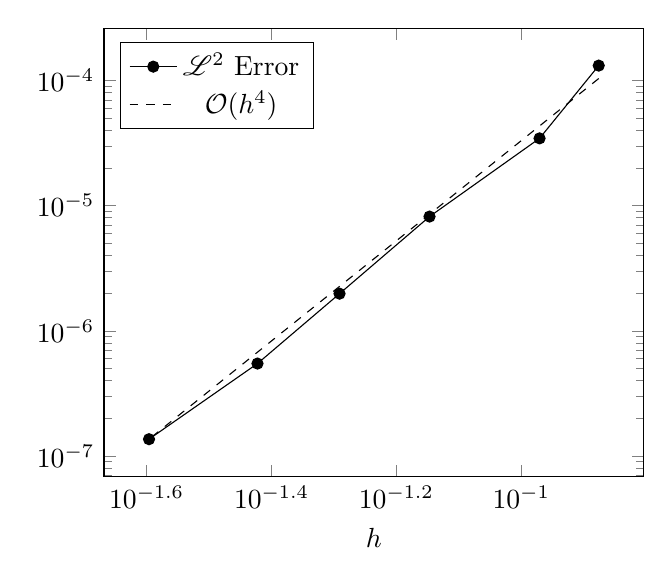
\begin{tikzpicture}
\begin{loglogaxis}[
    xlabel={$h$},
    legend pos=north west,
]

\addplot[black, mark=*] coordinates {(0.13307,0.000131393) (0.106989,3.44649e-05) (0.0713092,8.1769e-06) (0.0511671,1.98114e-06) (0.0378115,5.47747e-07) (0.0253431,1.36302e-07)};
\addlegendentry{$\LT$ Error}

\addplot[black, dashed] coordinates {(0.13307,0.0001036057614569891) (0.0253431,1.36302e-07)};
\addlegendentry{$\mathcal{O}(h^{4})$}

\end{loglogaxis}
\end{tikzpicture}
\end{subfigure}
\hfill
\begin{subfigure}[b]{0.45\textwidth}
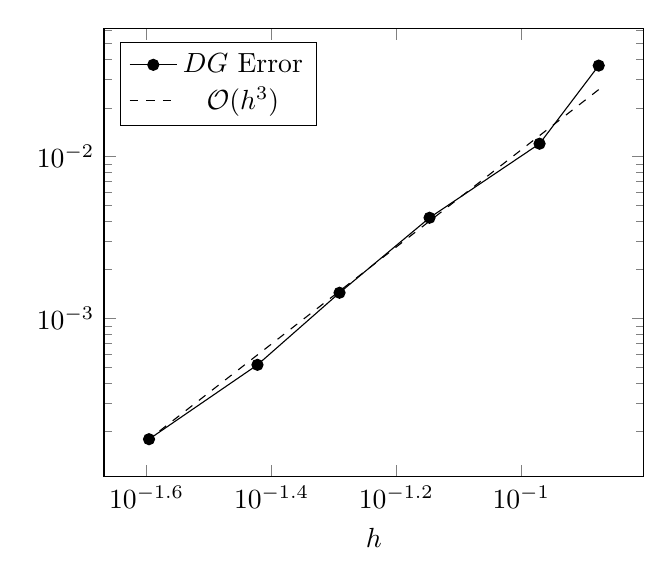
\begin{tikzpicture}
\begin{loglogaxis}[
    xlabel={$h$},
    legend pos=north west,
]

\addplot[black, mark=*] coordinates {(0.13307,0.036557) (0.106989,0.0120258) (0.0713092,0.00419264) (0.0511671,0.00144215) (0.0378115,0.000517054) (0.0253431,0.000179452)};
\addlegendentry{$DG$ Error}

\addplot[black, dashed] coordinates {(0.13307,0.025978230256595083) (0.0253431,0.000179452)};
\addlegendentry{$\mathcal{O}(h^{3})$}

\end{loglogaxis}
\end{tikzpicture}
\end{subfigure}
        \caption{$\LT$ and $DG$ errors versus mesh size on a sequence of uniform meshes over a square domain. $k = 3$, $N \in \{125, 250, \dots, 4000\}$.}
    \end{figure}
\end{frame}

\begin{frame}[fragile]
    \frametitle{Errors}
    \framesubtitle{L-shaped domain, smooth solution}

    \lstinline{./executables/lshape_smooth.out 3}

    \begin{figure}[!ht]
        % Errors v Size template for TikZ.

\begin{subfigure}[b]{0.45\textwidth}
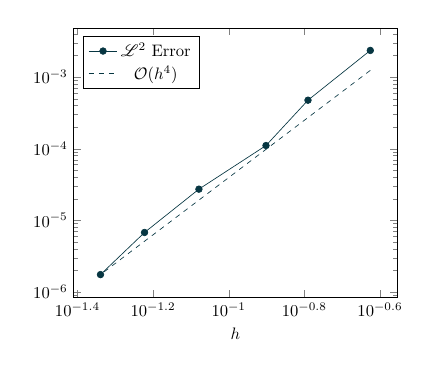
\begin{tikzpicture}[scale=.6]
\begin{loglogaxis}[
    xlabel={$h$},
    legend pos=north west,
]

\addplot[solarized-base02, mark=*] coordinates {(0.236846,0.00236589) (0.162063,0.000476832) (0.125487,0.000110835) (0.0834066,2.72149e-05) (0.0598985,6.75002e-06) (0.0458041,1.74035e-06)};
\addlegendentry{$\LT$ Error}

\addplot[solarized-base02, dashed] coordinates {(0.236846,0.0012441805245544592) (0.0458041,1.74035e-06)};
\addlegendentry{$\mathcal{O}(h^{4})$}

\end{loglogaxis}
\end{tikzpicture}
\end{subfigure}
\hfill
\begin{subfigure}[b]{0.45\textwidth}
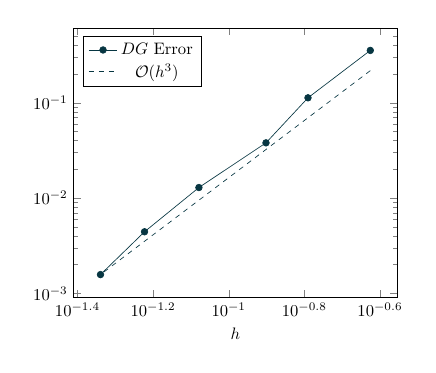
\begin{tikzpicture}[scale=.6]
\begin{loglogaxis}[
    xlabel={$h$},
    legend pos=north west,
]

\addplot[solarized-base02, mark=*] coordinates {(0.236846,0.354304) (0.162063,0.112679) (0.125487,0.0379581) (0.0834066,0.0128848) (0.0598985,0.00442298) (0.0458041,0.0015715)};
\addlegendentry{$DG$ Error}

\addplot[solarized-base02, dashed] coordinates {(0.236846,0.2172698609297559) (0.0458041,0.0015715)};
\addlegendentry{$\mathcal{O}(h^{3})$}

\end{loglogaxis}
\end{tikzpicture}
\end{subfigure}
        \caption{$\LT$ and $DG$ errors versus mesh size on a sequence of uniform meshes over an L-shaped domain. $k = 3$, $N \in \{125, 250, \dots, 4000\}$.}
    \end{figure}
\end{frame}

\begin{frame}[fragile]
    \frametitle{Errors}
    \framesubtitle{Square domain, low-regularity solution}

    \lstinline{./executables/square.out 3}

    \begin{figure}[!ht]
        % Errors v Size template for TikZ.

\begin{subfigure}[b]{0.45\textwidth}
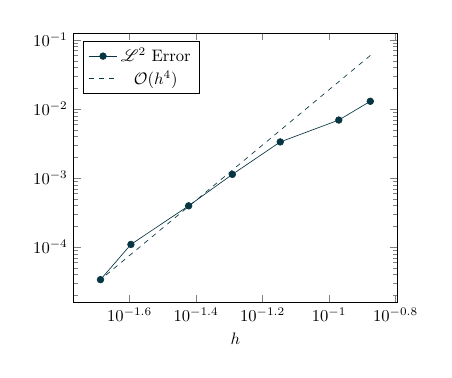
\begin{tikzpicture}[scale=.6]
\begin{loglogaxis}[
    xlabel={$h$},
    legend pos=north west,
]

\addplot[solarized-base02, mark=*] coordinates {(0.13307,0.0129373) (0.106989,0.00691892) (0.0713092,0.00333505) (0.0511671,0.0011295) (0.0378115,0.000395856) (0.0253431,0.000109201) (0.0205266,3.37306e-05)};
\addlegendentry{$\LT$ Error}

\addplot[solarized-base02, dashed] coordinates {(0.13307,0.05957672373397235) (0.0205266,3.37306e-05)};
\addlegendentry{$\mathcal{O}(h^{4})$}

\end{loglogaxis}
\end{tikzpicture}
\end{subfigure}
\hfill
\begin{subfigure}[b]{0.45\textwidth}
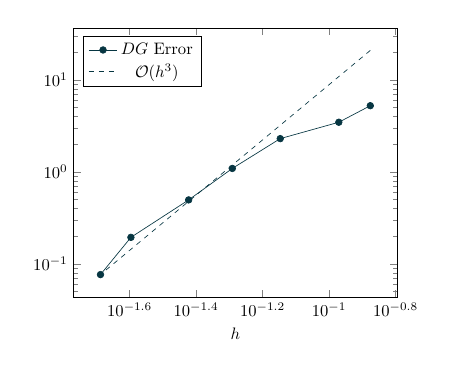
\begin{tikzpicture}[scale=.6]
\begin{loglogaxis}[
    xlabel={$h$},
    legend pos=north west,
]

\addplot[solarized-base02, mark=*] coordinates {(0.13307,5.22824) (0.106989,3.45593) (0.0713092,2.29411) (0.0511671,1.08811) (0.0378115,0.495229) (0.0253431,0.194102) (0.0205266,0.0764724)};
\addlegendentry{$DG$ Error}

\addplot[solarized-base02, dashed] coordinates {(0.13307,20.83503013128883) (0.0205266,0.0764724)};
\addlegendentry{$\mathcal{O}(h^{3})$}

\end{loglogaxis}
\end{tikzpicture}
\end{subfigure}
        \caption{$\LT$ and $DG$ errors versus mesh size on a sequence of uniform meshes over a square domain. $k = 3$, $N \in \{125, 250, \dots, 8000\}$.}
    \end{figure}
\end{frame}

\begin{frame}[fragile]
    \frametitle{Errors}
    \framesubtitle{L-shaped domain, low-regularity solution}

    \lstinline{./executables/lshape.out 3}

    \begin{figure}[!ht]
        % Errors v Size template for TikZ.

\begin{subfigure}[b]{0.45\textwidth}
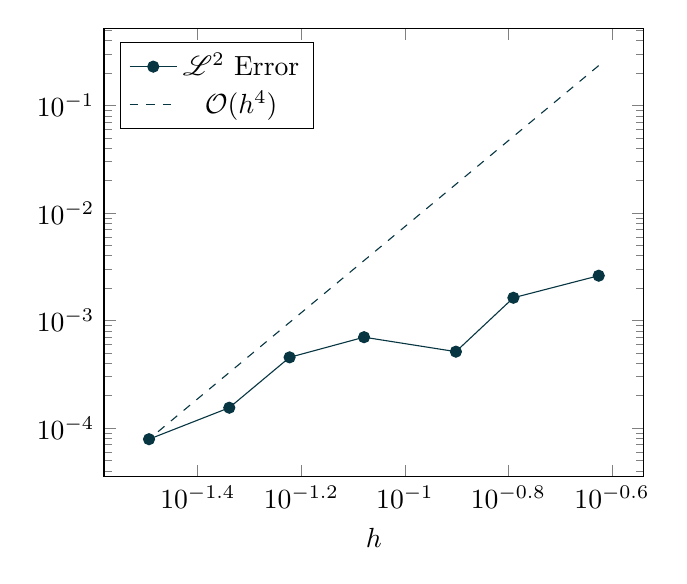
\begin{tikzpicture}
\begin{loglogaxis}[
    xlabel={$h$},
    legend pos=north west,
]

\addplot[solarized-base02, mark=*] coordinates {(0.236846,0.00261101) (0.162063,0.00162784) (0.125487,0.000513351) (0.0834066,0.000699775) (0.0598985,0.000454435) (0.0458041,0.000154545) (0.0320544,7.87786e-05)};
\addlegendentry{$\LT$ Error}

\addplot[solarized-base02, dashed] coordinates {(0.236846,0.23481285454935658) (0.0320544,7.87786e-05)};
\addlegendentry{$\mathcal{O}(h^{4})$}

\end{loglogaxis}
\end{tikzpicture}
\end{subfigure}
\hfill
\begin{subfigure}[b]{0.45\textwidth}
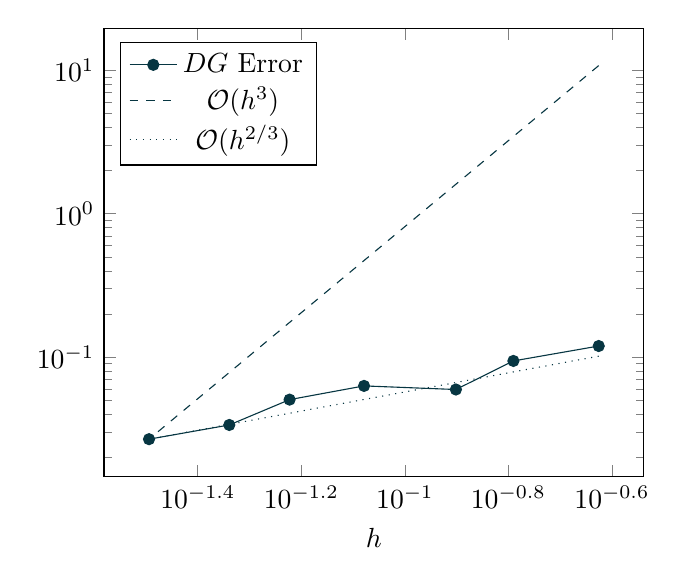
\begin{tikzpicture}
\begin{loglogaxis}[
    xlabel={$h$},
    legend pos=north west,
]

\addplot[solarized-base02, mark=*] coordinates {(0.236846,0.119546) (0.162063,0.0940845) (0.125487,0.0594576) (0.0834066,0.0630073) (0.0598985,0.0505441) (0.0458041,0.0336456) (0.0320544,0.0267768)};
\addlegendentry{$DG$ Error}

\addplot[solarized-base02, dashed] coordinates {(0.236846,10.801744041106874) (0.0320544,0.0267768)};
\addlegendentry{$\mathcal{O}(h^{3})$}

\addplot[solarized-base02, dotted] coordinates {(0.236846,0.10158063960750381) (0.0320544,0.0267768)};
\addlegendentry{$\mathcal{O}(h^{2/3})$}

\end{loglogaxis}
\end{tikzpicture}
\end{subfigure}
        \caption{$\LT$ and $DG$ errors versus mesh size on a sequence of uniform meshes over an L-shaped domain. $k = 3$, $N \in \{125, 250, \dots, 8000\}$.}
    \end{figure}
\end{frame}

\begin{frame}
    \frametitle{Meshes}

    \begin{figure}[!ht]
        \centering
        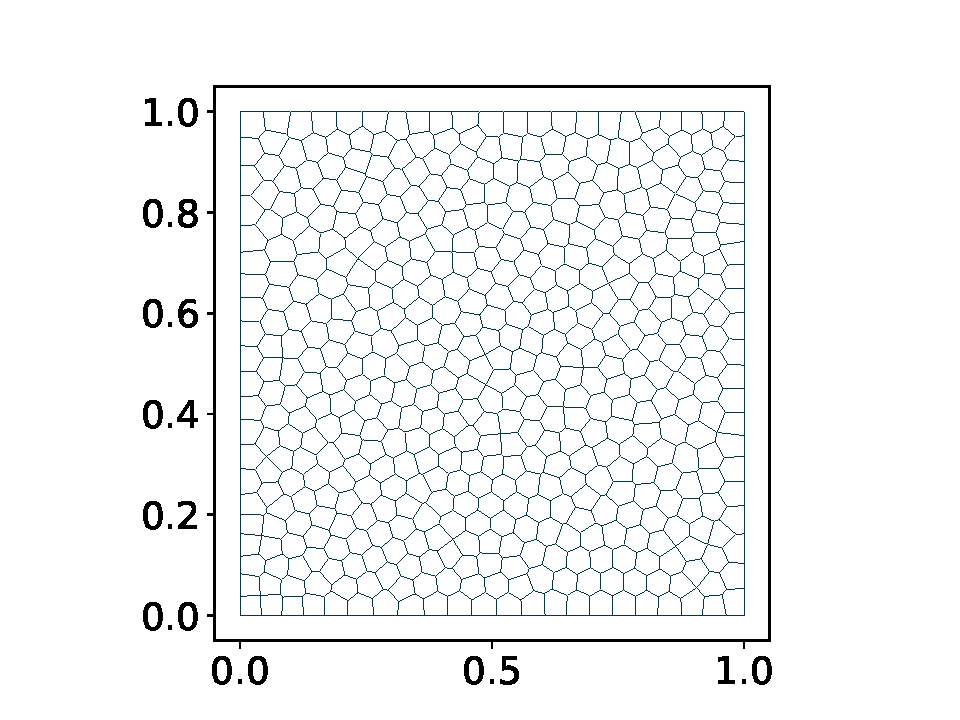
\includegraphics[trim=1cm 0.5cm 1cm 0.5cm, clip, width=0.275\textwidth]{meshes/uniform/square_500.pdf}
        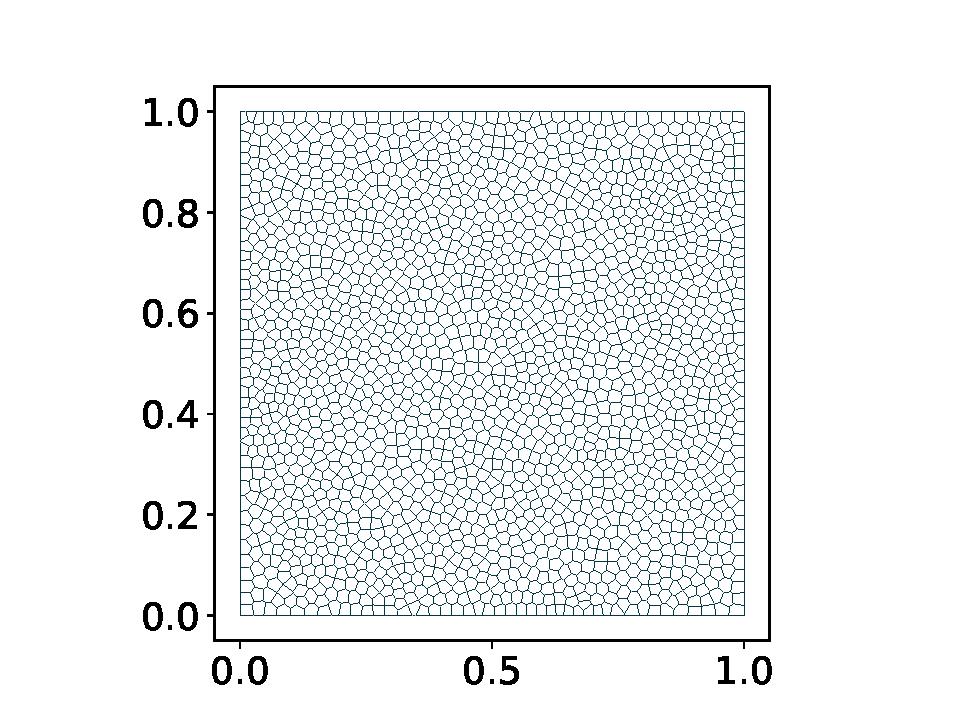
\includegraphics[trim=1cm 0.5cm 1cm 0.5cm, clip, width=0.275\textwidth]{meshes/uniform/square_2000.pdf}
        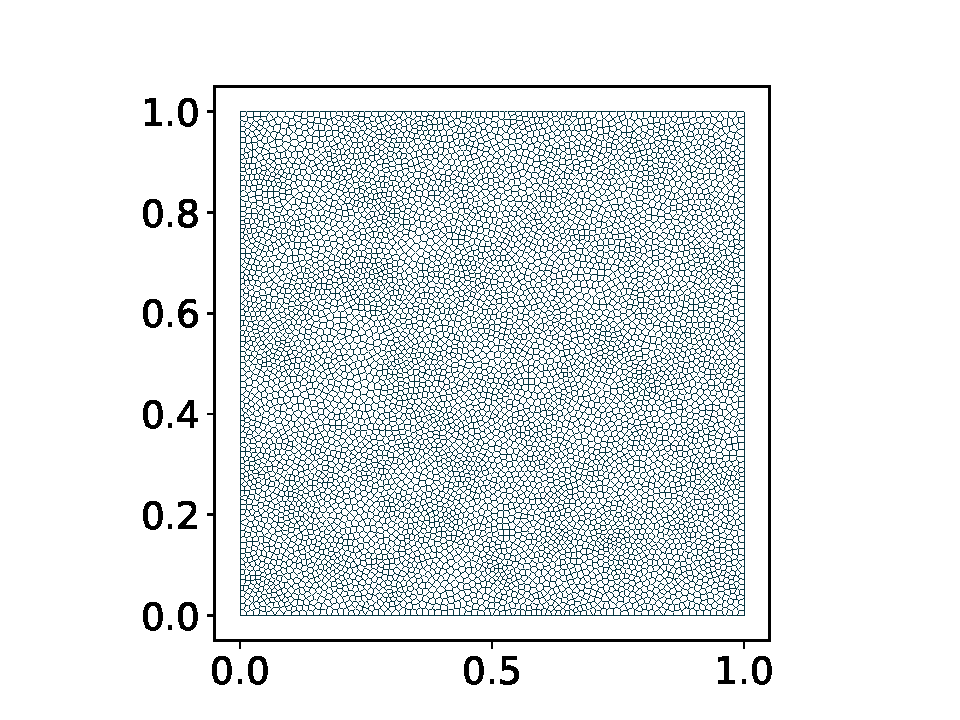
\includegraphics[trim=1cm 0.5cm 1cm 0.5cm, clip, width=0.275\textwidth]{meshes/uniform/square_8000.pdf}
        \caption{Square uniform meshes, with $N \in \{500, 2000, 8000\}$.}
    \end{figure}

    \begin{figure}[!ht]
        \centering
        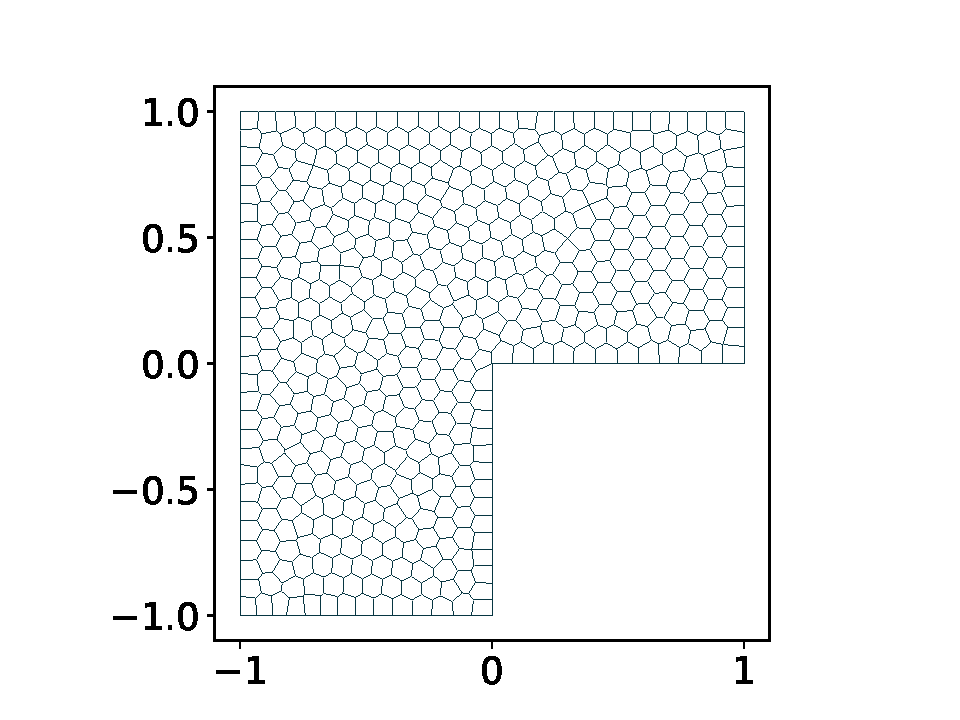
\includegraphics[trim=1cm 0.5cm 1cm 0.5cm, clip, width=0.275\textwidth]{meshes/uniform/lshape_500.pdf}
        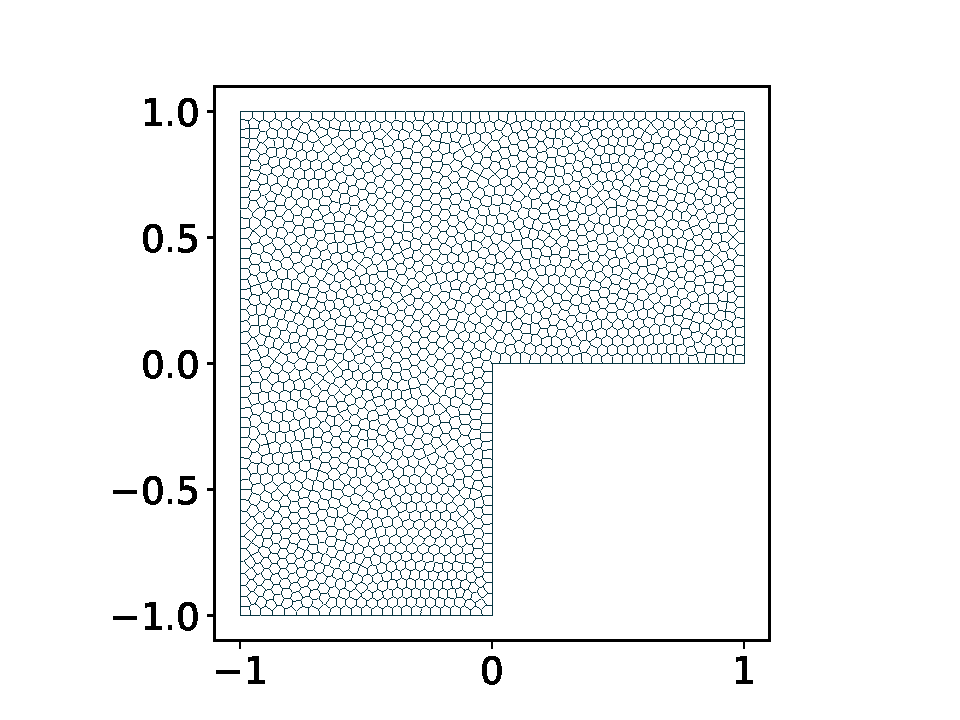
\includegraphics[trim=1cm 0.5cm 1cm 0.5cm, clip, width=0.275\textwidth]{meshes/uniform/lshape_2000.pdf}
        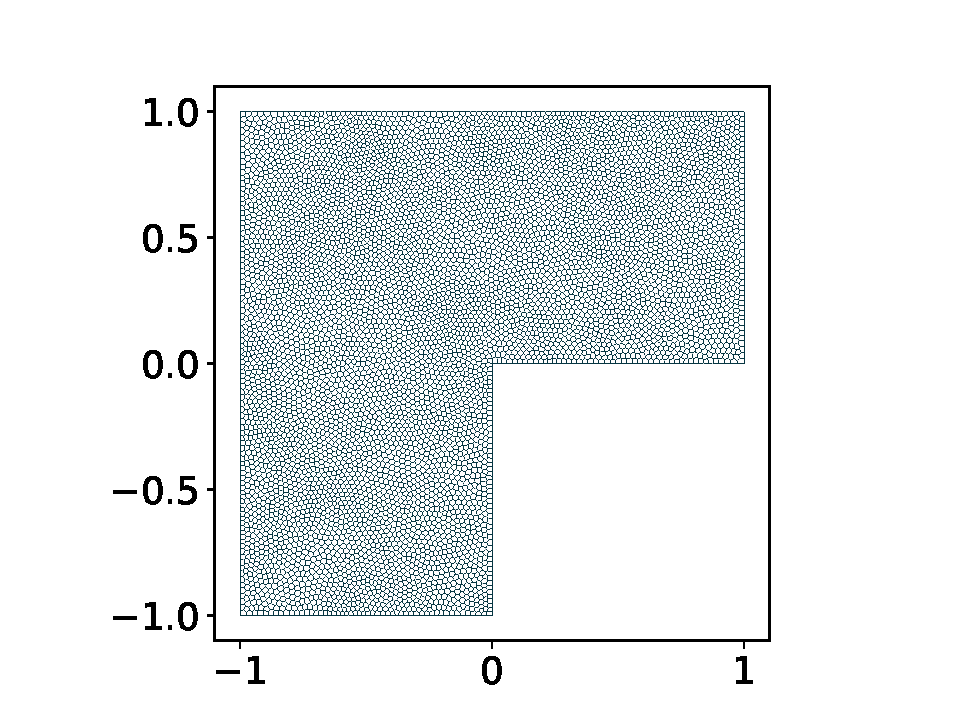
\includegraphics[trim=1cm 0.5cm 1cm 0.5cm, clip, width=0.275\textwidth]{meshes/uniform/lshape_8000.pdf}
        \caption{L-shaped uniform meshes, with $N \in \{500, 2000, 8000\}$.}
    \end{figure}
\end{frame}

\subsection{Uniform Refinement Versus \textit{h-Adaptive} Refinement}

\begin{frame}[fragile]
    \frametitle{Errors}
    \framesubtitle{Both domains, $\LT$ errors}

    \lstinline{./executables/square_h.out 3 125}
    \lstinline{./executables/lshape_h.out 3 125}

    \begin{figure}[!ht]
        \begin{subfigure}[b]{0.45\textwidth}
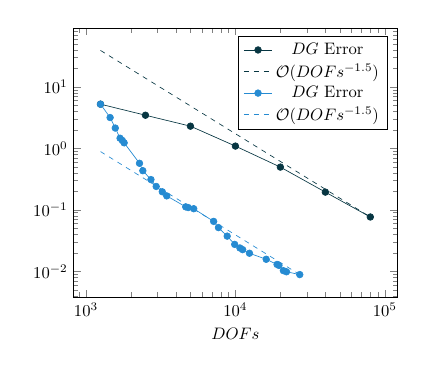
\begin{tikzpicture}[scale=.6]
\begin{loglogaxis}[
    xlabel={$DOFs$},
    legend pos=north east,
]

\addplot[solarized-base02, mark=*] coordinates {(1250,5.22824) (2500,3.45593) (5000,2.29411) (10000,1.08811) (20000,0.495229) (40000,0.194102) (80000,0.0764724)};
\addlegendentry{$DG$ Error}

\addplot[solarized-base02, dashed] coordinates {(1250,39.1538688) (80000,0.0764724)};
\addlegendentry{$\mathcal{O}(DOFs^{-1.5})$}

\addplot[\accentcolor, mark=*] coordinates {(1250,5.22824) (1450,3.16847) (1570,2.13764) (1690,1.46207) (1750,1.34315) (1800,1.22937) (2280,0.571535) (2400,0.433165) (2720,0.310514) (2950,0.239953) (3240,0.196515) (3470,0.168581) (4650,0.111757) (4830,0.108861) (5260,0.104274) (7150,0.0648557) (7700,0.0513934) (8810,0.0373304) (9890,0.0273954) (10720,0.0239574) (11180,0.0225082) (12420,0.0196702) (16070,0.0156938) (19010,0.0129343) (19560,0.0124709) (20950,0.0102387) (21970,0.00982763) (26960,0.00884522)};
\addlegendentry{$DG$ Error}

\addplot[\accentcolor, dashed] coordinates {(1250,0.8859790477668384) (26960,0.00884522)};
\addlegendentry{$\mathcal{O}(DOFs^{-1.5})$}

\end{loglogaxis}
\end{tikzpicture}
\end{subfigure}
\hfill
\begin{subfigure}[b]{0.45\textwidth}
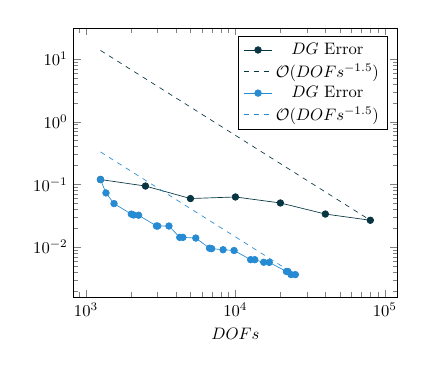
\begin{tikzpicture}[scale=.6]
\begin{loglogaxis}[
    xlabel={$DOFs$},
    legend pos=north east,
]

\addplot[solarized-base02, mark=*] coordinates {(1250,0.119546) (2500,0.0940843) (5000,0.0594572) (10000,0.0630071) (20000,0.050544) (40000,0.0336455) (80000,0.0267768)};
\addlegendentry{$DG$ Error}

\addplot[solarized-base02, dashed] coordinates {(1250,13.7097216) (80000,0.0267768)};
\addlegendentry{$\mathcal{O}(DOFs^{-1.5})$}

\addplot[\accentcolor, mark=*] coordinates {(1250,0.119546) (1360,0.0730976) (1540,0.0493759) (2010,0.0335623) (2080,0.0325106) (2250,0.0322421) (2960,0.0217044) (3020,0.0216543) (3590,0.0216774) (4240,0.0142896) (4450,0.0142875) (5430,0.0139307) (6710,0.009591) (6930,0.0094454) (8270,0.00907011) (9800,0.00881814) (12650,0.00629972) (13480,0.00629107) (15470,0.00572756) (16850,0.00569782) (21960,0.00407968) (22460,0.00407912) (23570,0.00364227) (25190,0.00363907)};
\addlegendentry{$DG$ Error}

\addplot[\accentcolor, dashed] coordinates {(1250,0.3292059237674489) (25190,0.00363907)};
\addlegendentry{$\mathcal{O}(DOFs^{-1.5})$}

\end{loglogaxis}
\end{tikzpicture}
\end{subfigure}
        \caption{$DG$ errors versus $DOFs$ comparison between adaptively refined meshes and a sequence of uniform meshes over a square domain (left) and an L-shaped domain (right). $k = 3$, $N_0 = 125$.}
    \end{figure}
\end{frame}

\begin{frame}
    \frametitle{Meshes}

    \begin{figure}[!ht]
        \centering
        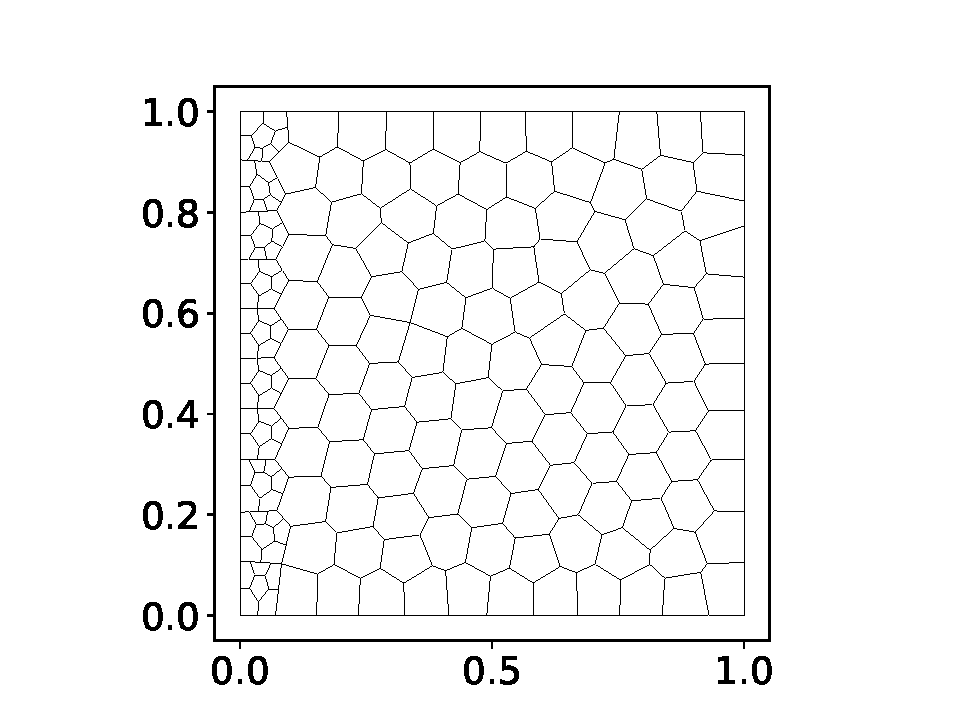
\includegraphics[trim=1cm 0.5cm 1cm 0.5cm, clip, width=0.275\textwidth]{meshes/adaptive/square_h_5.pdf}
        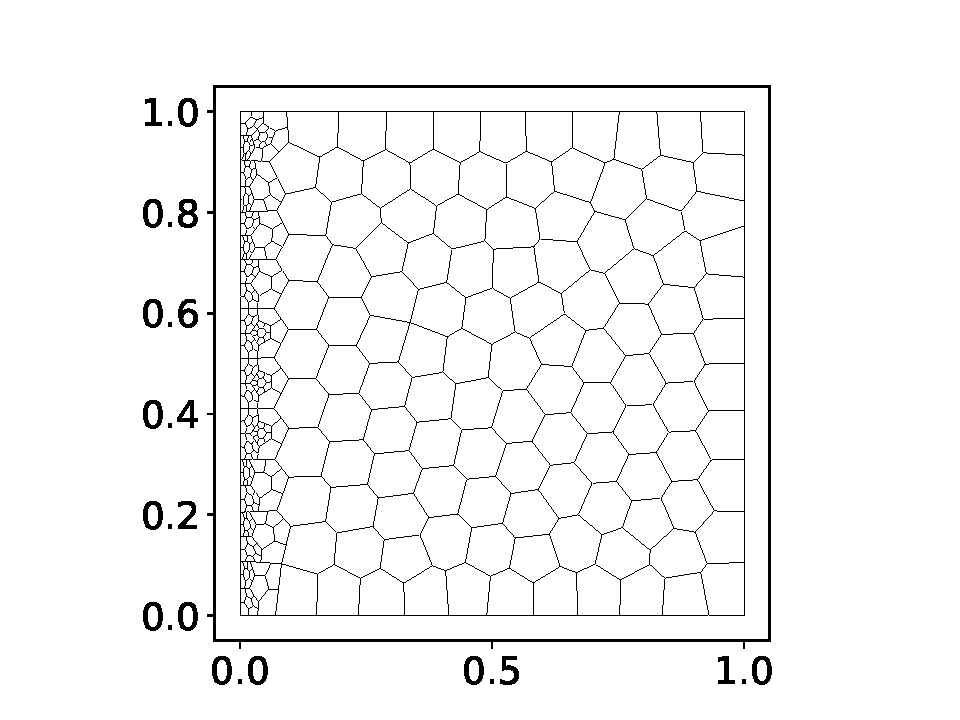
\includegraphics[trim=1cm 0.5cm 1cm 0.5cm, clip, width=0.275\textwidth]{meshes/adaptive/square_h_10.pdf}
        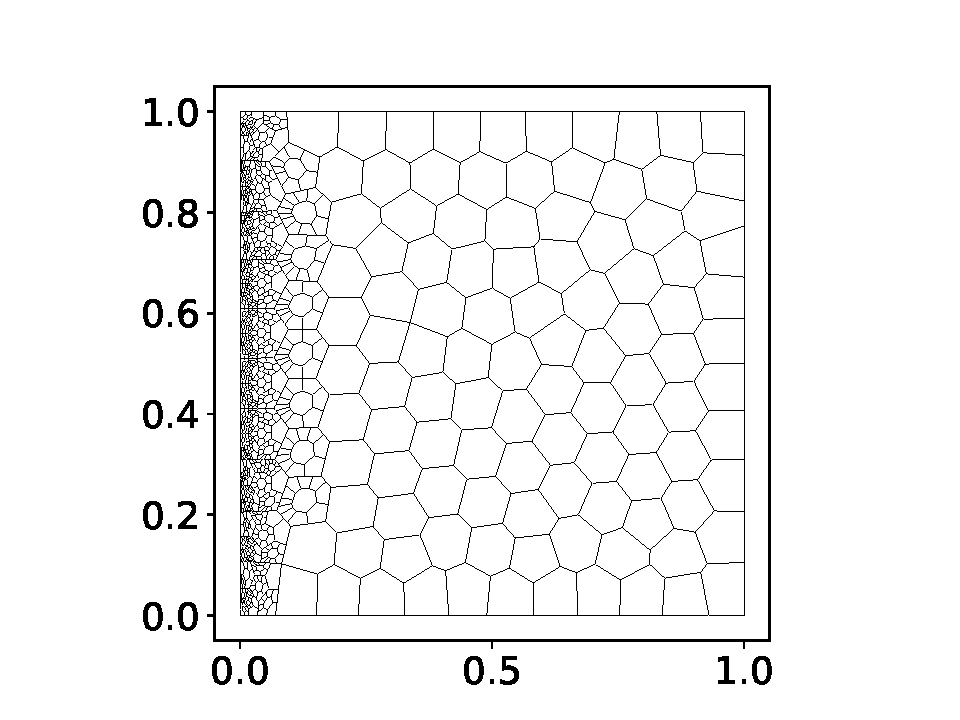
\includegraphics[trim=1cm 0.5cm 1cm 0.5cm, clip, width=0.275\textwidth]{meshes/adaptive/square_h_20.pdf}
        \caption{Square mesh after 5, 10, and 20 refinements, $N_0 = 125$.}
    \end{figure}
    
    \begin{figure}[!ht]
        \centering
        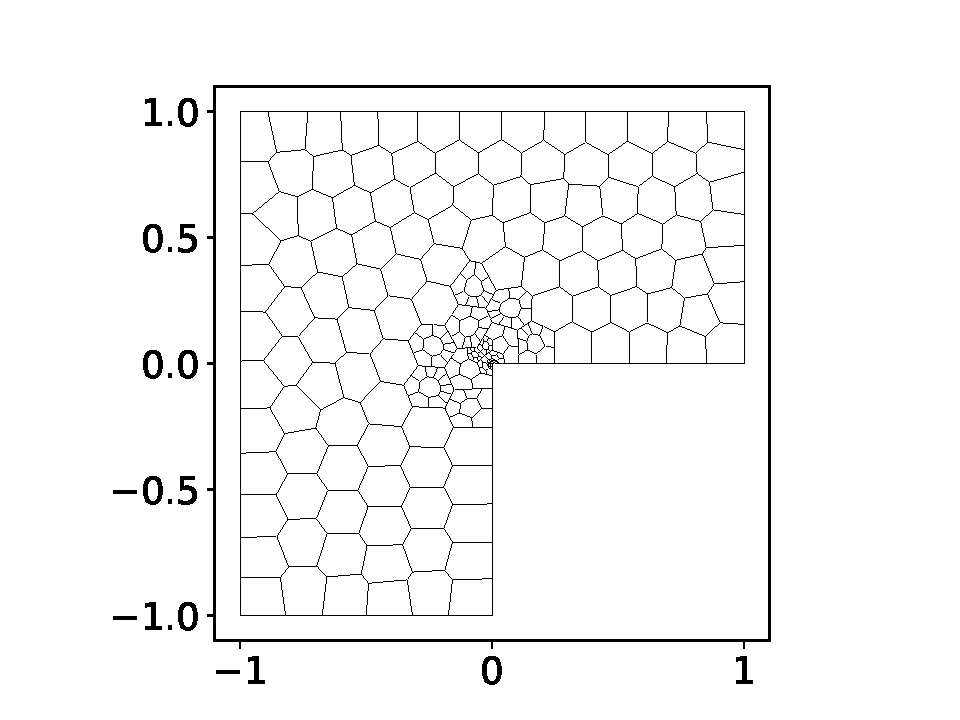
\includegraphics[trim=1cm 0.5cm 1cm 0.5cm, clip, width=0.275\textwidth]{meshes/adaptive/lshape_h_5.pdf}
        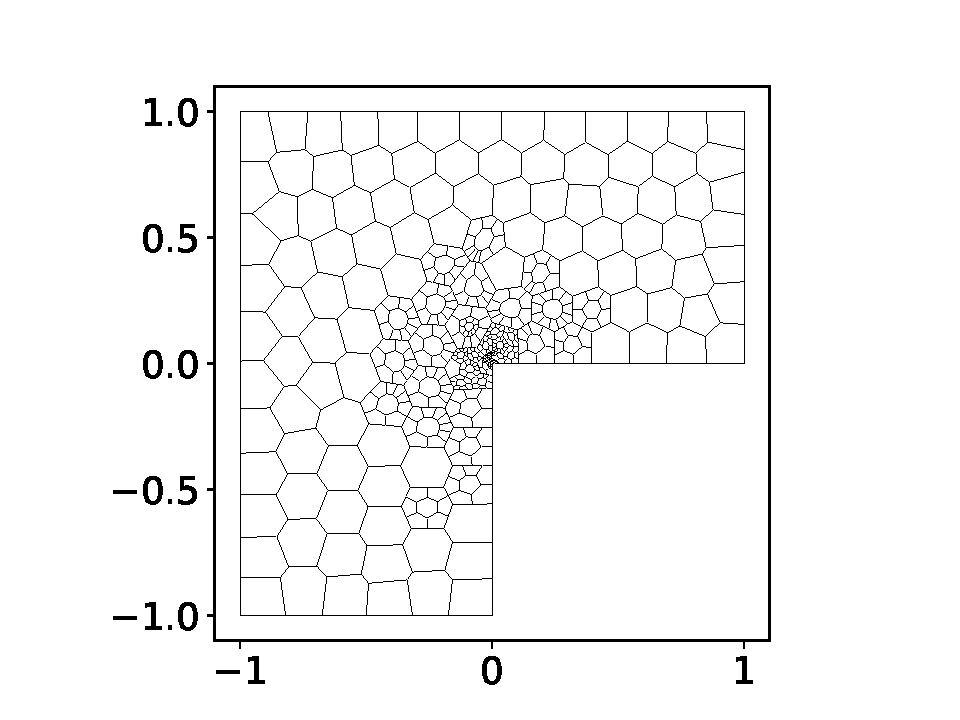
\includegraphics[trim=1cm 0.5cm 1cm 0.5cm, clip, width=0.275\textwidth]{meshes/adaptive/lshape_h_10.pdf}
        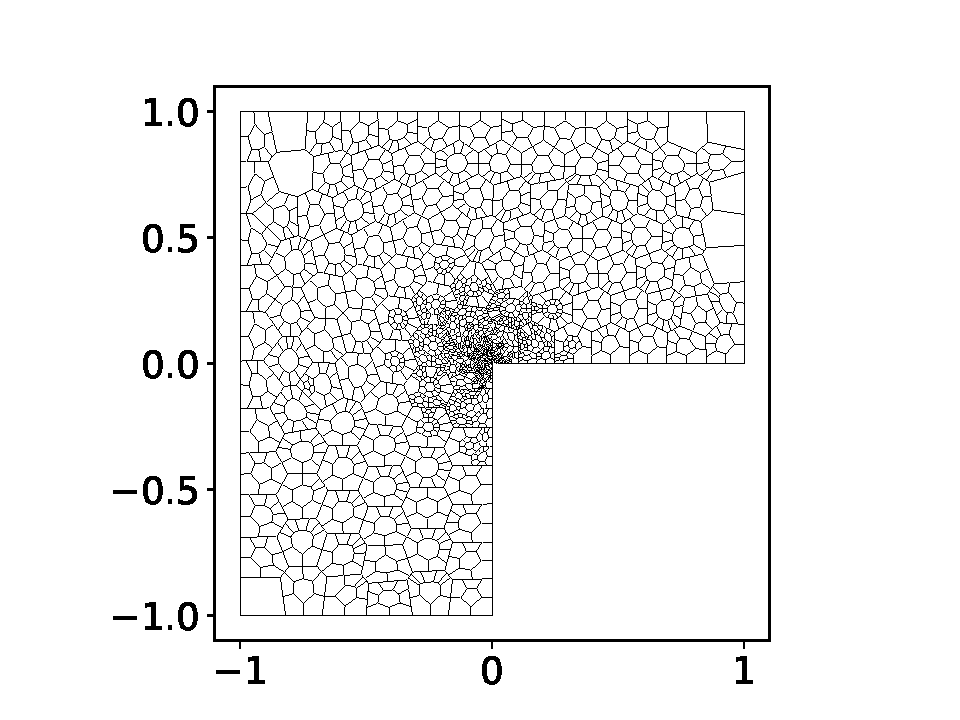
\includegraphics[trim=1cm 0.5cm 1cm 0.5cm, clip, width=0.275\textwidth]{meshes/adaptive/lshape_h_20.pdf}
        \caption{L-shaped mesh after 5, 10, and 20 refinements, $N_0 = 125$.}
    \end{figure}
\end{frame}

\begin{frame}[fragile]
    \frametitle{Errors}
    \framesubtitle{Both domains, $\HO$ errors}

    \lstinline{./executables/square_gh.out 3 125}
    \lstinline{./executables/lshape_gh.out 3 125}

    \begin{figure}[!ht]
        \begin{subfigure}[b]{0.45\textwidth}
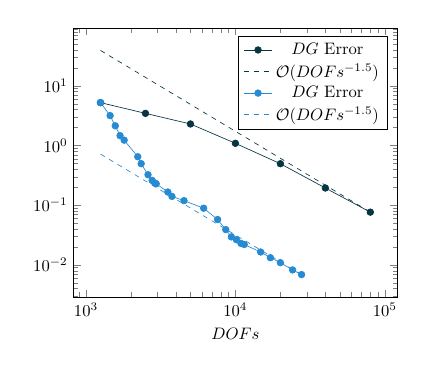
\begin{tikzpicture}[scale=.6]
\begin{loglogaxis}[
    xlabel={$DOFs$},
    legend pos=north east,
]

\addplot[solarized-base02, mark=*] coordinates {(1250,5.22824) (2500,3.45593) (5000,2.29411) (10000,1.08811) (20000,0.495229) (40000,0.194102) (80000,0.0764724)};
\addlegendentry{$DG$ Error}

\addplot[solarized-base02, dashed] coordinates {(1250,39.1538688) (80000,0.0764724)};
\addlegendentry{$\mathcal{O}(DOFs^{-1.5})$}

\addplot[\accentcolor, mark=*] coordinates {(1250,5.22824) (1450,3.16847) (1570,2.13764) (1690,1.46207) (1800,1.22937) (2220,0.648223) (2340,0.495982) (2600,0.323852) (2770,0.260152) (2880,0.236183) (2950,0.22874) (3530,0.166199) (3760,0.140521) (4530,0.119187) (6130,0.089056) (7600,0.0575574) (8620,0.0390489) (9400,0.0294453) (10160,0.0263927) (10900,0.0229053) (11450,0.0219544) (14750,0.0164373) (17150,0.0131901) (19990,0.0109056) (24140,0.00823295) (27720,0.00688026)};
\addlegendentry{$DG$ Error}

\addplot[\accentcolor, dashed] coordinates {(1250,0.7185047930727512) (27720,0.00688026)};
\addlegendentry{$\mathcal{O}(DOFs^{-1.5})$}

\end{loglogaxis}
\end{tikzpicture}
\end{subfigure}
\hfill
\begin{subfigure}[b]{0.45\textwidth}
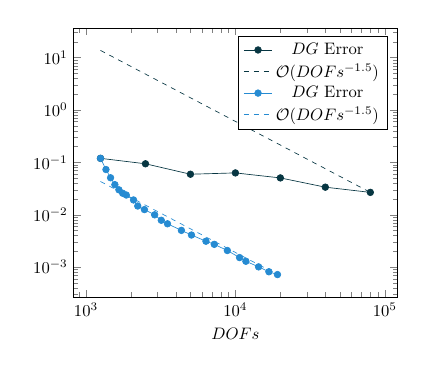
\begin{tikzpicture}[scale=.6]
\begin{loglogaxis}[
    xlabel={$DOFs$},
    legend pos=north east,
]

\addplot[solarized-base02, mark=*] coordinates {(1250,0.119546) (2500,0.0940843) (5000,0.0594572) (10000,0.0630071) (20000,0.050544) (40000,0.0336455) (80000,0.0267768)};
\addlegendentry{$DG$ Error}

\addplot[solarized-base02, dashed] coordinates {(1250,13.7097216) (80000,0.0267768)};
\addlegendentry{$\mathcal{O}(DOFs^{-1.5})$}

\addplot[\accentcolor, mark=*] coordinates {(1250,0.119546) (1360,0.0730976) (1460,0.0508708) (1560,0.0375773) (1660,0.0299764) (1760,0.0257653) (1860,0.0238484) (2080,0.0191889) (2220,0.0147015) (2460,0.0125616) (2880,0.00998454) (3190,0.00786125) (3510,0.00673439) (4350,0.0050375) (5080,0.00411082) (6350,0.00313077) (7220,0.00272903) (8830,0.00208062) (10660,0.0015255) (11750,0.00129659) (14290,0.00101426) (16760,0.000817683) (19120,0.00072222)};
\addlegendentry{$DG$ Error}

\addplot[\accentcolor, dashed] coordinates {(1250,0.04320523018854778) (19120,0.00072222)};
\addlegendentry{$\mathcal{O}(DOFs^{-1.5})$}

\end{loglogaxis}
\end{tikzpicture}
\end{subfigure}
        \caption{$DG$ errors versus $DOFs$ comparison between adaptively refined meshes and a sequence of uniform meshes over a square domain (left) and an L-shaped domain (right). $k = 3$, $N_0 = 125$.}
    \end{figure}
\end{frame}

\begin{frame}
    \frametitle{Meshes}

\begin{figure}[!ht]
    \centering
    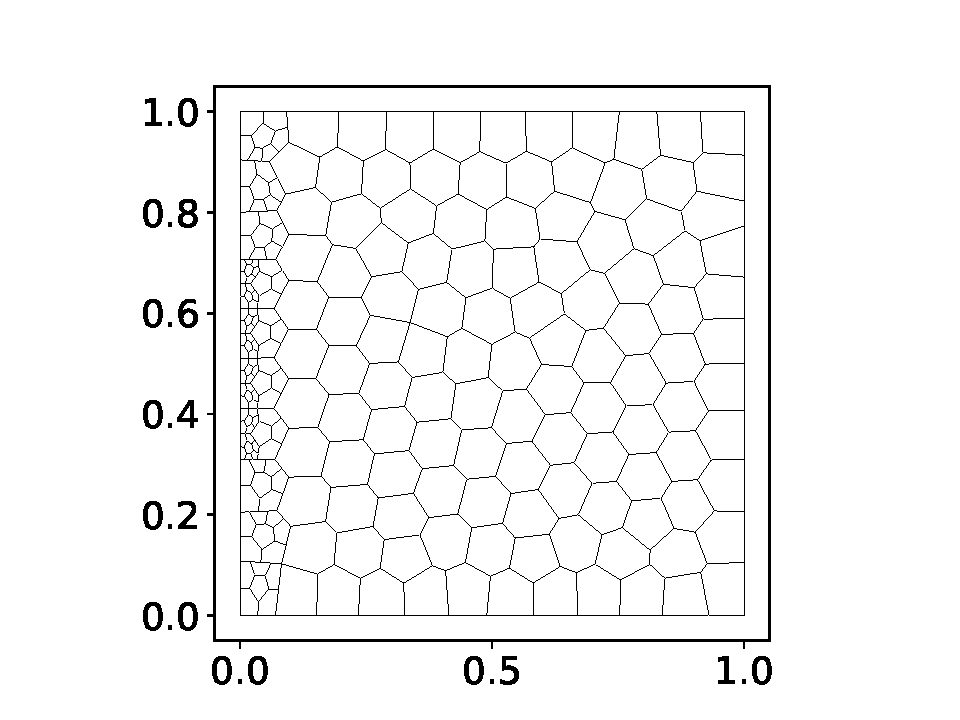
\includegraphics[trim=1cm 0.5cm 1cm 0.5cm, clip, width=0.275\textwidth]{meshes/adaptive/square_gh_5.pdf}
    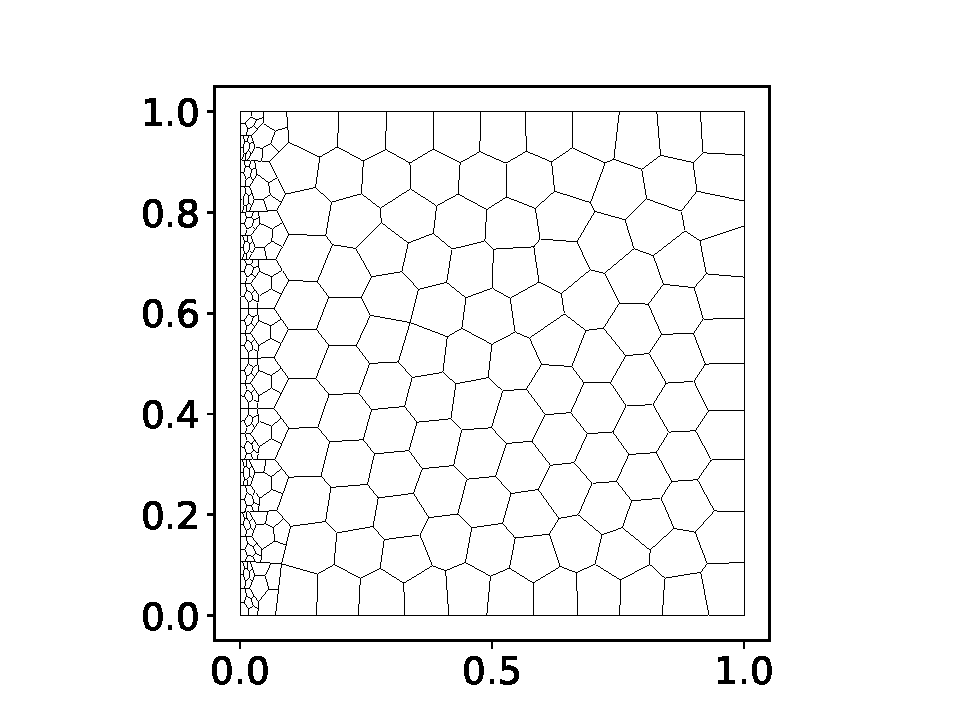
\includegraphics[trim=1cm 0.5cm 1cm 0.5cm, clip, width=0.275\textwidth]{meshes/adaptive/square_gh_10.pdf}
    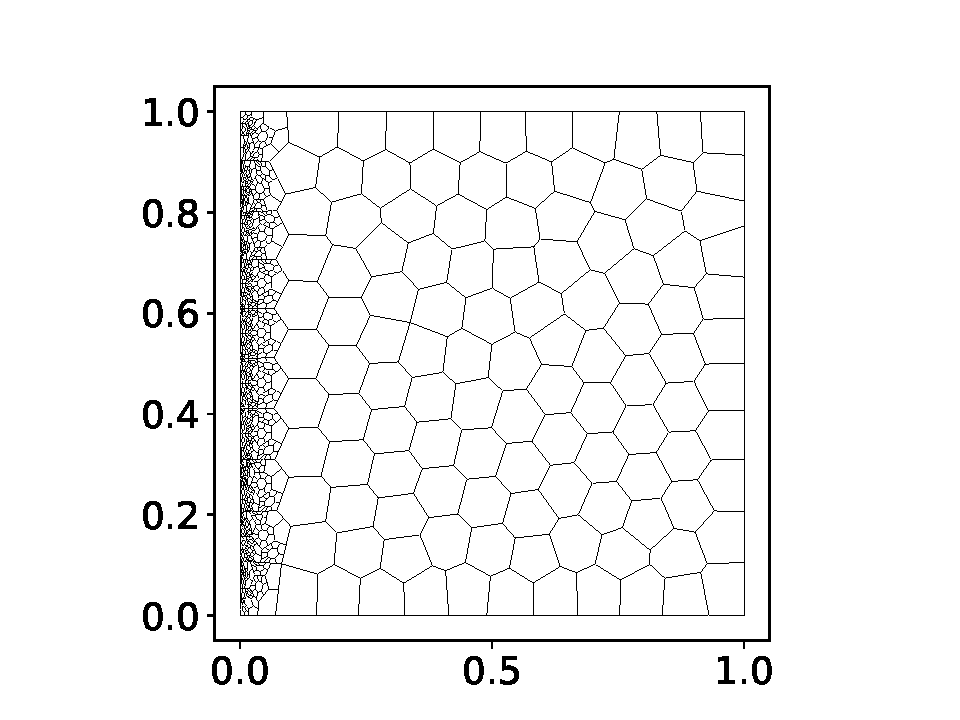
\includegraphics[trim=1cm 0.5cm 1cm 0.5cm, clip, width=0.275\textwidth]{meshes/adaptive/square_gh_20.pdf}
    \caption{Square mesh after 5, 10, and 20 refinements, $N_0 = 125$.}
\end{figure}

\begin{figure}[!ht]
    \centering
    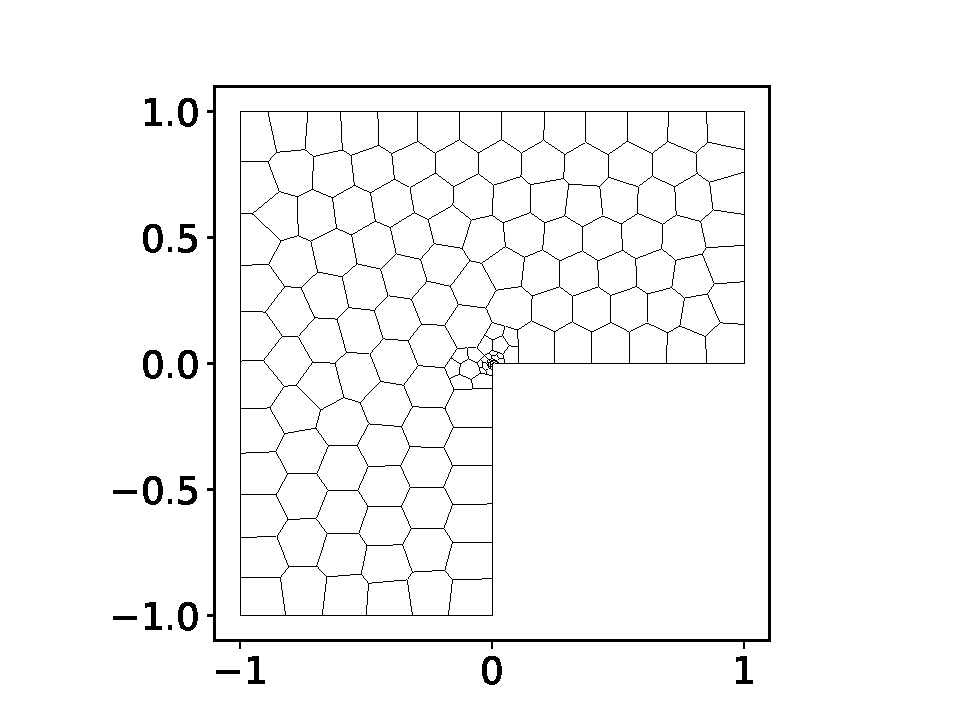
\includegraphics[trim=1cm 0.5cm 1cm 0.5cm, clip, width=0.275\textwidth]{meshes/adaptive/lshape_gh_5.pdf}
    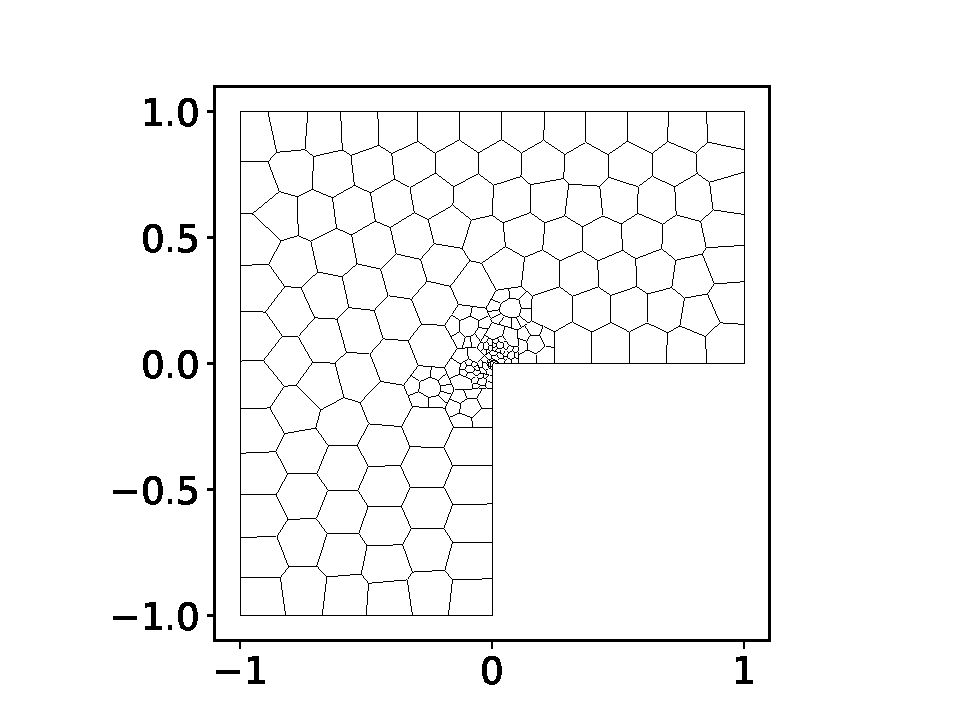
\includegraphics[trim=1cm 0.5cm 1cm 0.5cm, clip, width=0.275\textwidth]{meshes/adaptive/lshape_gh_10.pdf}
    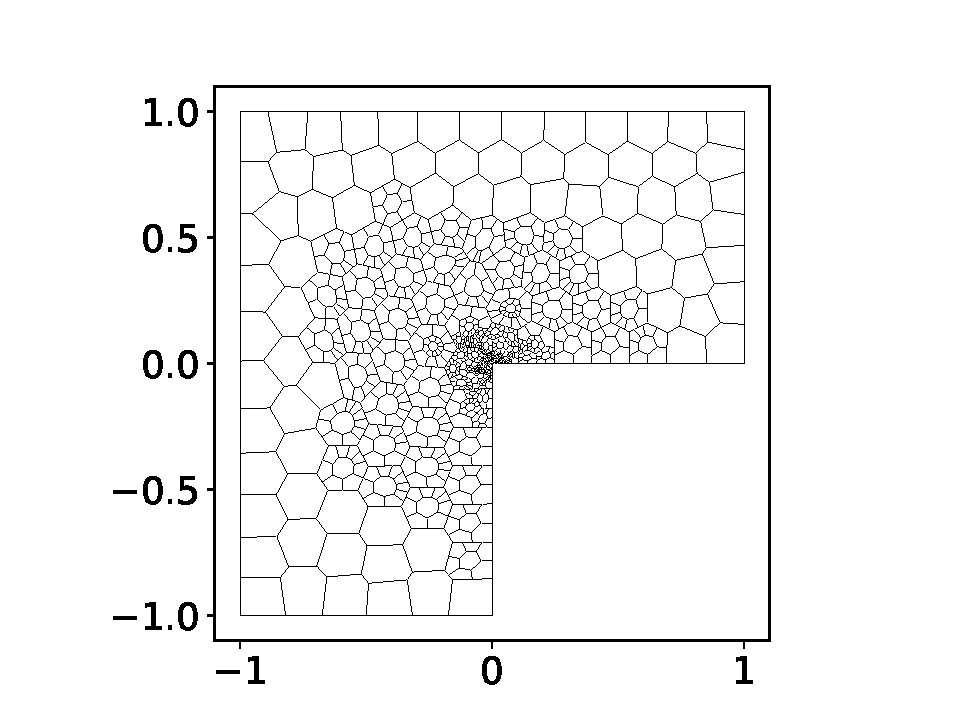
\includegraphics[trim=1cm 0.5cm 1cm 0.5cm, clip, width=0.275\textwidth]{meshes/adaptive/lshape_gh_20.pdf}
    \caption{L-shaped mesh after 5, 10, and 20 refinements, $N_0 = 125$.}
\end{figure}
\end{frame}

\begin{frame}[fragile]
    \frametitle{Errors}
    \framesubtitle{Both domains, estimator}

    \lstinline{./executables/square_eh.out 3 125}
    \lstinline{./executables/lshape_eh.out 3 125}

    \begin{figure}[!ht]
        \begin{subfigure}[b]{0.45\textwidth}
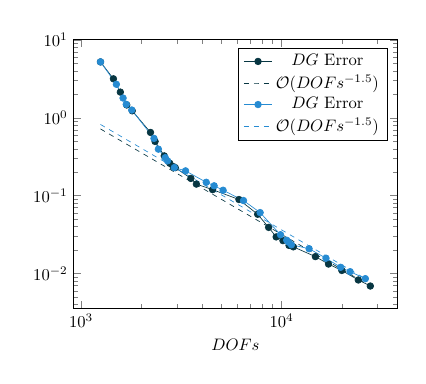
\begin{tikzpicture}[scale=.6]
\begin{loglogaxis}[
    xlabel={$DOFs$},
    legend pos=north east,
]

\addplot[solarized-base02, mark=*] coordinates {(1250,5.22824) (1450,3.16847) (1570,2.13764) (1690,1.46207) (1800,1.22937) (2220,0.648223) (2340,0.495982) (2600,0.323852) (2770,0.260152) (2880,0.236183) (2950,0.22874) (3530,0.166199) (3760,0.140521) (4530,0.119187) (6130,0.089056) (7600,0.0575574) (8620,0.0390489) (9400,0.0294453) (10160,0.0263927) (10900,0.0229053) (11450,0.0219544) (14750,0.0164373) (17150,0.0131901) (19990,0.0109056) (24140,0.00823295) (27720,0.00688026)};
\addlegendentry{$DG$ Error}

\addplot[solarized-base02, dashed] coordinates {(1250,0.7185047930727512) (27720,0.00688026)};
\addlegendentry{$\mathcal{O}(DOFs^{-1.5})$}

\addplot[\accentcolor, mark=*] coordinates {(1250,5.22824) (1500,2.69514) (1620,1.7934) (1680,1.48702) (1790,1.25894) (2310,0.543447) (2430,0.395368) (2630,0.307434) (2700,0.279644) (2920,0.229209) (3320,0.207952) (4210,0.148303) (4610,0.133591) (5110,0.117099) (6460,0.0863494) (7820,0.0604748) (9880,0.0314321) (10610,0.0267064) (10850,0.0251548) (11200,0.0233236) (13720,0.0207803) (16660,0.0156883) (19710,0.0119851) (21980,0.0105234) (26180,0.00856227)};
\addlegendentry{$DG$ Error}

\addplot[\accentcolor, dashed] coordinates {(1250,0.8206885275389775) (26180,0.00856227)};
\addlegendentry{$\mathcal{O}(DOFs^{-1.5})$}

\end{loglogaxis}
\end{tikzpicture}
\end{subfigure}
\hfill
\begin{subfigure}[b]{0.45\textwidth}
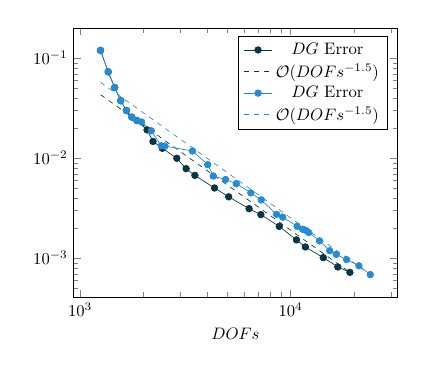
\begin{tikzpicture}[scale=.6]
\begin{loglogaxis}[
    xlabel={$DOFs$},
    legend pos=north east,
]

\addplot[solarized-base02, mark=*] coordinates {(1250,0.119546) (1360,0.0730976) (1460,0.0508708) (1560,0.0375773) (1660,0.0299764) (1760,0.0257653) (1860,0.0238484) (2080,0.0191889) (2220,0.0147015) (2460,0.0125616) (2880,0.00998454) (3190,0.00786125) (3510,0.00673439) (4350,0.0050375) (5080,0.00411082) (6350,0.00313077) (7220,0.00272903) (8830,0.00208062) (10660,0.0015255) (11750,0.00129659) (14290,0.00101426) (16760,0.000817683) (19120,0.00072222)};
\addlegendentry{$DG$ Error}

\addplot[solarized-base02, dashed] coordinates {(1250,0.04320523018854778) (19120,0.00072222)};
\addlegendentry{$\mathcal{O}(DOFs^{-1.5})$}

\addplot[\accentcolor, mark=*] coordinates {(1250,0.119546) (1360,0.0730976) (1460,0.0508708) (1560,0.0375773) (1660,0.0299764) (1760,0.0257653) (1860,0.0238484) (1960,0.0230301) (2180,0.0187842) (2430,0.0133021) (2530,0.0132102) (3420,0.0118042) (4040,0.00861783) (4290,0.00663868) (4910,0.00612195) (5520,0.00556495) (6470,0.00450029) (7250,0.00383231) (8580,0.00274332) (9170,0.00257528) (10740,0.00208511) (11390,0.0019513) (11790,0.00190163) (12190,0.0018094) (13720,0.00149002) (15340,0.00118862) (16470,0.00109125) (18450,0.000969034) (21110,0.000840165) (23910,0.000686294)};
\addlegendentry{$DG$ Error}

\addplot[\accentcolor, dashed] coordinates {(1250,0.05741356925713827) (23910,0.000686294)};
\addlegendentry{$\mathcal{O}(DOFs^{-1.5})$}

\end{loglogaxis}
\end{tikzpicture}
\end{subfigure}
        \caption{$DG$ errors versus $DOFs$ comparison between adaptively refined meshes over a square domain (left) and an L-shaped domain (right). $k = 3$, $N_0 = 125$.}
    \end{figure}
\end{frame}

\begin{frame}
    \frametitle{Meshes}

    \begin{figure}[!ht]
        \centering
        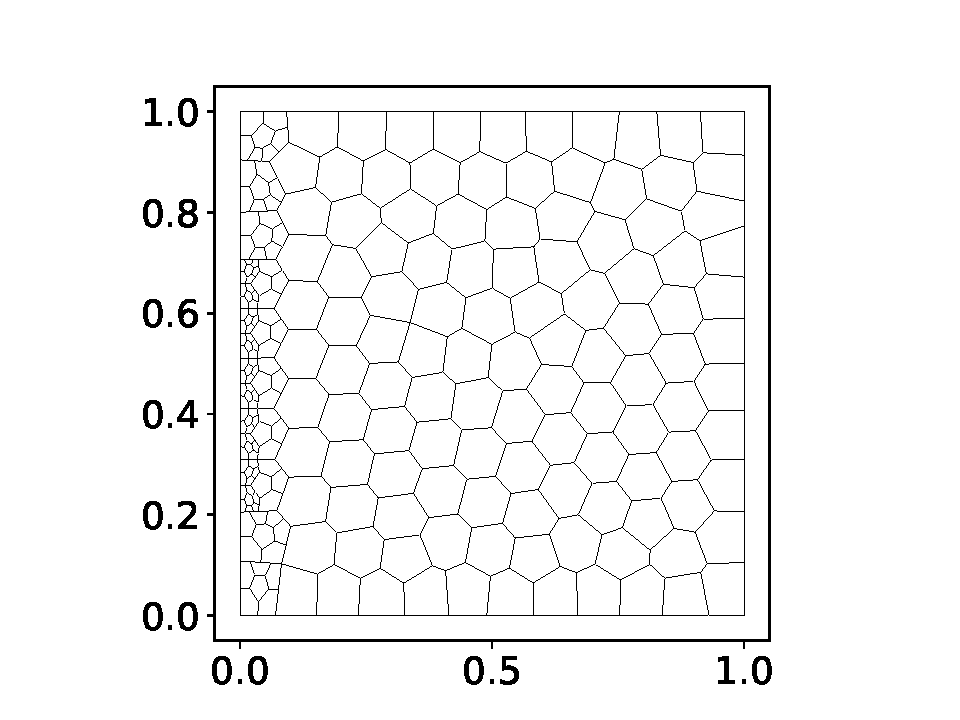
\includegraphics[trim=1cm 0.5cm 1cm 0.5cm, clip, width=0.275\textwidth]{meshes/adaptive/square_eh_5.pdf}
        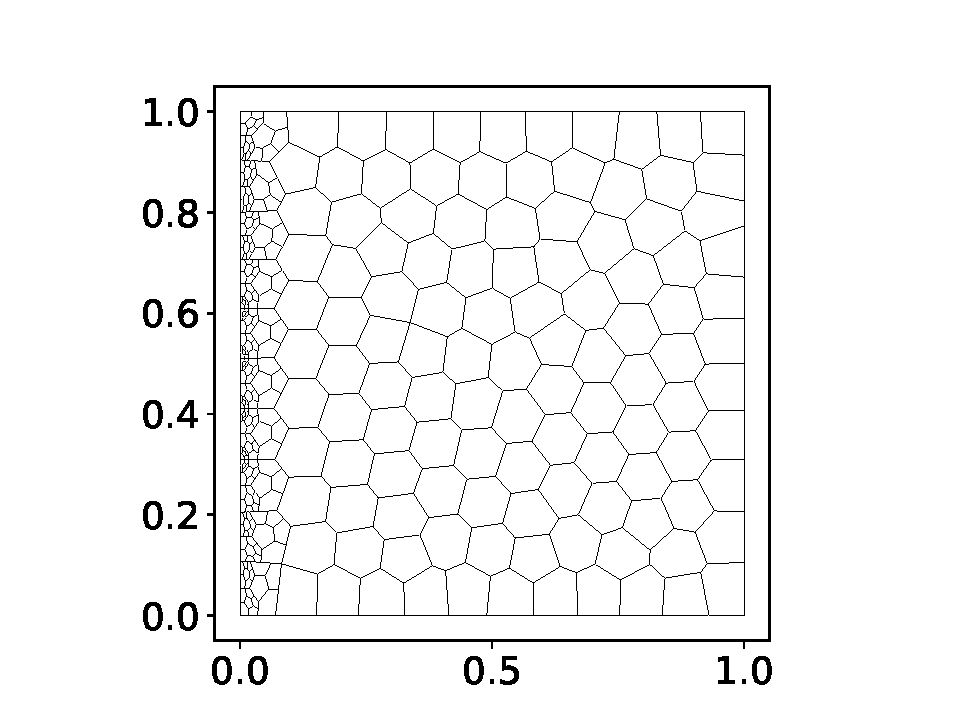
\includegraphics[trim=1cm 0.5cm 1cm 0.5cm, clip, width=0.275\textwidth]{meshes/adaptive/square_eh_10.pdf}
        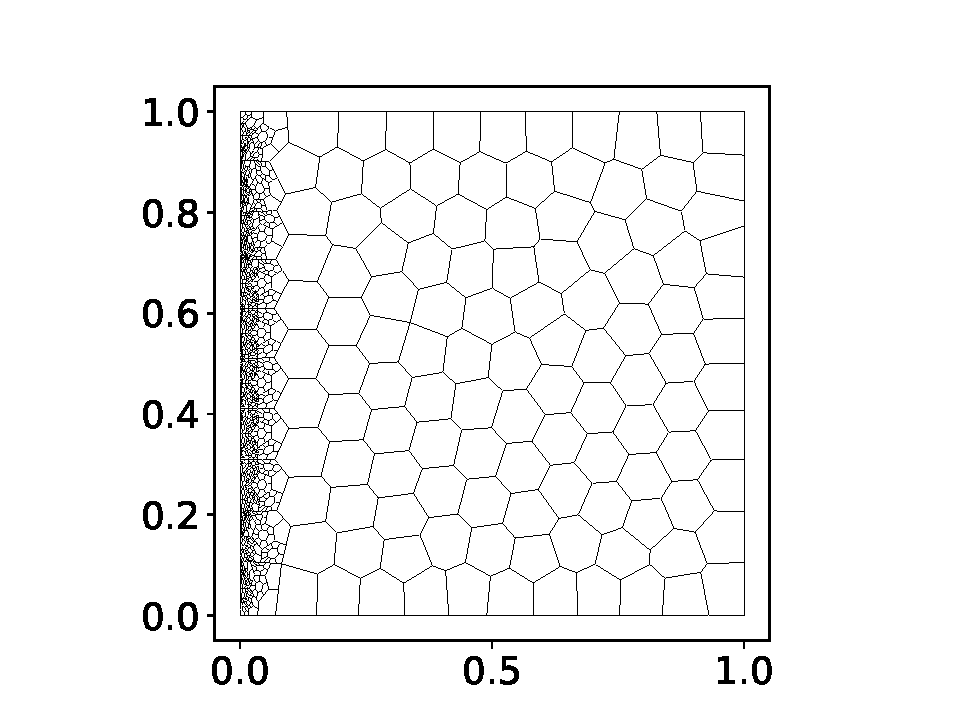
\includegraphics[trim=1cm 0.5cm 1cm 0.5cm, clip, width=0.275\textwidth]{meshes/adaptive/square_eh_20.pdf}
        \caption{Square mesh after 5, 10, and 20 refinements, $N_0 = 125$.}
    \end{figure}
    
    \begin{figure}[!ht]
        \centering
        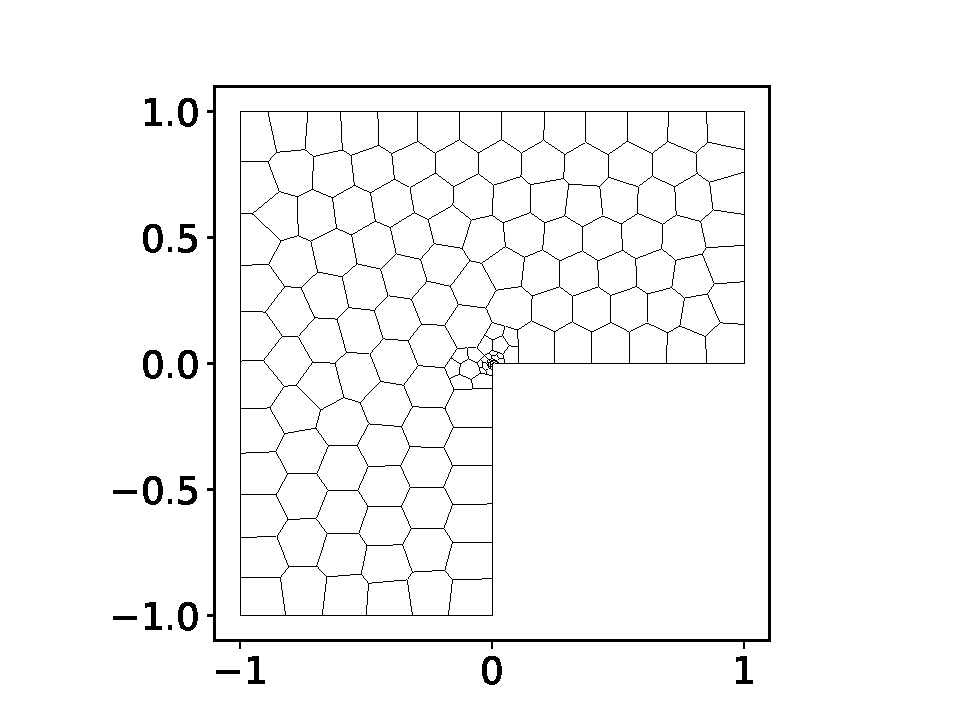
\includegraphics[trim=1cm 0.5cm 1cm 0.5cm, clip, width=0.275\textwidth]{meshes/adaptive/lshape_eh_5.pdf}
        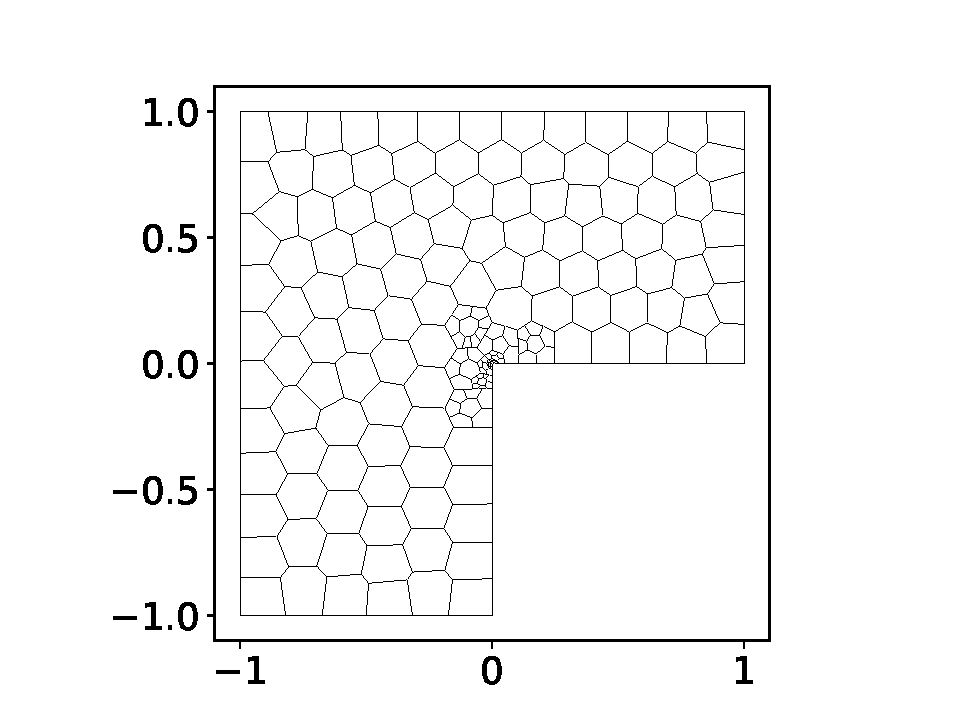
\includegraphics[trim=1cm 0.5cm 1cm 0.5cm, clip, width=0.275\textwidth]{meshes/adaptive/lshape_eh_10.pdf}
        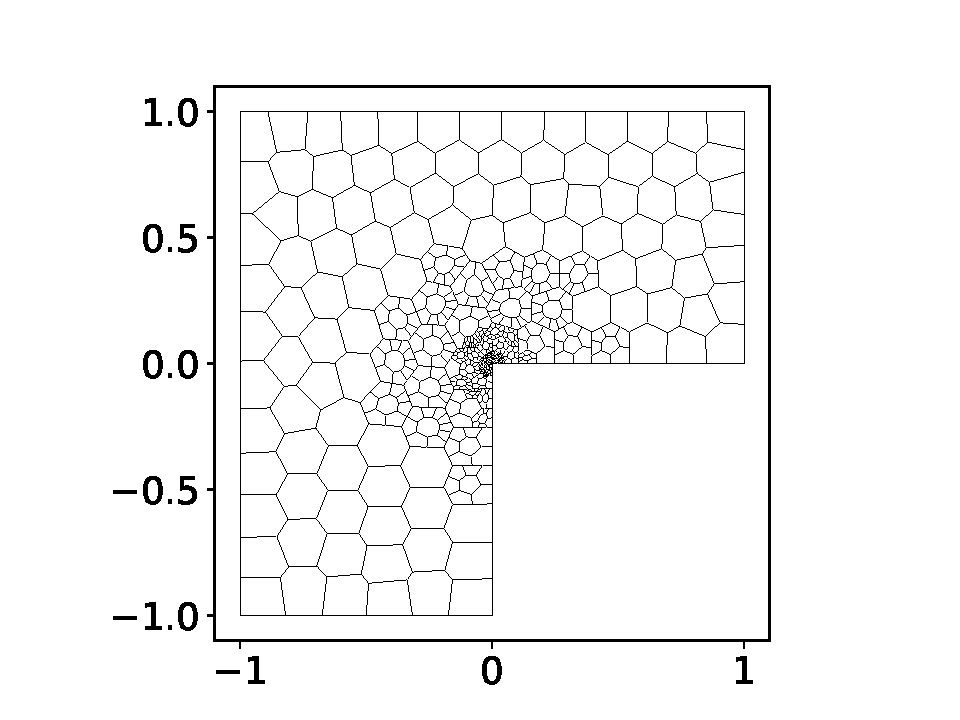
\includegraphics[trim=1cm 0.5cm 1cm 0.5cm, clip, width=0.275\textwidth]{meshes/adaptive/lshape_eh_20.pdf}
        \caption{L-shaped mesh after 5, 10, and 20 refinements, $N_0 = 125$.}
    \end{figure}
\end{frame}

\subsection{\textit{hp-Adaptive} Refinement}

\begin{frame}[fragile]
    \frametitle{Errors}
    \framesubtitle{Both domains}

    \lstinline{./executables/square_hp.out 1 25}
    \lstinline{./executables/lshape_hp.out 1 25}

    \begin{figure}[!ht]
        \begin{subfigure}[b]{0.45\textwidth}
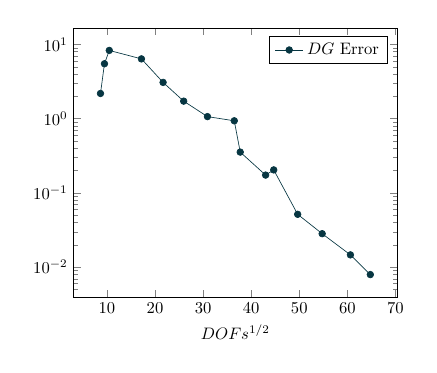
\begin{tikzpicture}[scale=.6]
\begin{axis}[
    xlabel={$DOFs^{1/2}$}, % Edit if needed.
    legend pos=north east,
    ymode=log
]

\addplot[solarized-base02, mark=*] coordinates {(8.660254037844387,2.1812) (9.486832980505138,5.48286) (10.488088481701515,8.28706) (17.175564037317667,6.37634) (21.6794833886788,3.07509) (25.96150997149434,1.71936) (30.903074280724887,1.06513) (36.4828726939094,0.935197) (37.72267222772003,0.3543) (43.0,0.173769) (44.68780594300866,0.204124) (49.66890375275057,0.0514923) (54.76312628037227,0.0282501) (60.63827174318213,0.0146515) (64.77653896280658,0.0079507)};
\addlegendentry{$DG$ Error}

\end{axis}
\end{tikzpicture}
\end{subfigure}
\hfill
\begin{subfigure}[b]{0.45\textwidth}
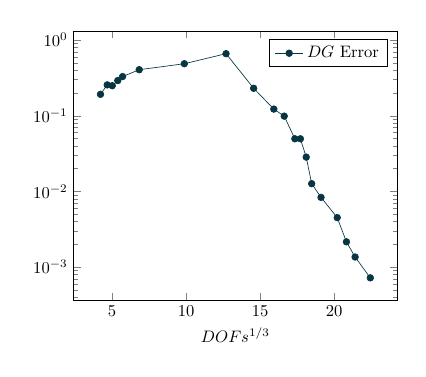
\begin{tikzpicture}[scale=.6]
\begin{axis}[
    xlabel={$DOFs^{1/3}$}, % Edit if needed.
    legend pos=north east,
    ymode=log
]

\addplot[solarized-base02, mark=*] coordinates {(4.217163326508746,0.191755) (4.672328728355259,0.255398) (5.0132979349645845,0.248801) (5.383212612087283,0.291174) (5.708267473384861,0.328607) (6.832771452246442,0.404871) (9.878530490026034,0.485699) (12.69507321245234,0.659013) (14.55901434377428,0.230073) (15.921490395218942,0.122269) (16.623800957486996,0.098664) (17.340316055801914,0.0495985) (17.714635665253457,0.0495794) (18.10839938601742,0.0283923) (18.477938151928672,0.0126687) (19.10925056502305,0.00835058) (20.20211721754757,0.00451385) (20.823924640400417,0.00216312) (21.4106622851008,0.00136207) (22.436197851201577,0.00072339)};
\addlegendentry{$DG$ Error}

\end{axis}
\end{tikzpicture}
\end{subfigure}
        \caption{$DG$ error versus $DOFs^{1/2}$ (left) and $DOFs^{1/3}$ (right) on a sequence of \textit{hp-adaptively} refined meshes over a square domain (left) and an L-shaped domain (right). $k_0 = 1$, $N_0 = 25$.}
    \end{figure}
\end{frame}

\begin{frame}
    \frametitle{Meshes}

    \begin{figure}[!ht]
        \centering
        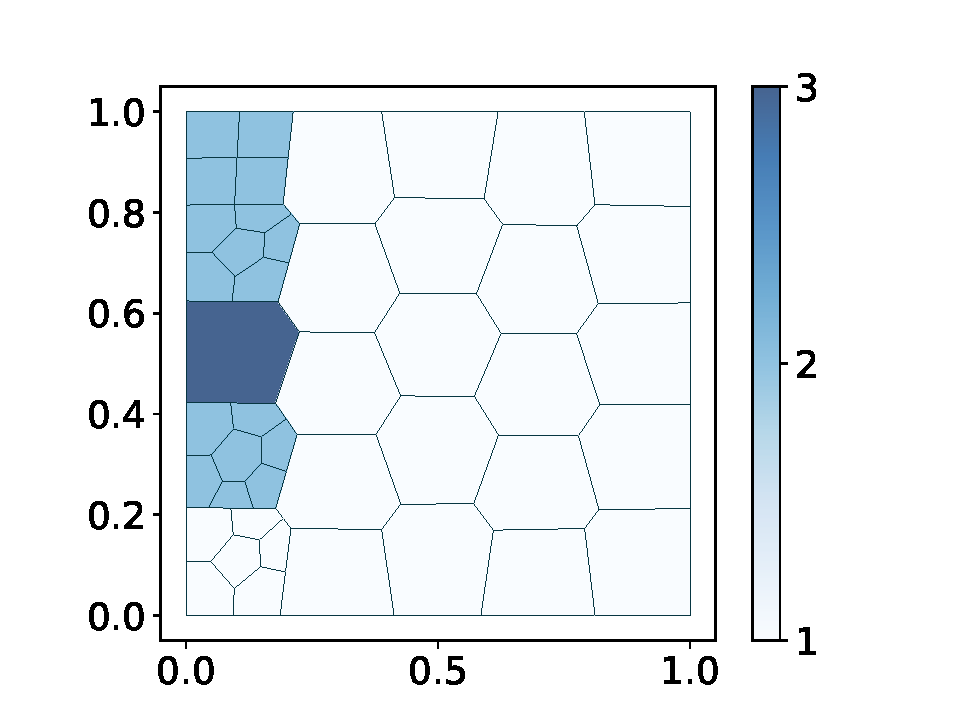
\includegraphics[trim=1cm 0.5cm 1cm 0.5cm, clip, width=0.275\textwidth]{meshes/adaptive/square_hp_1_2.pdf}
        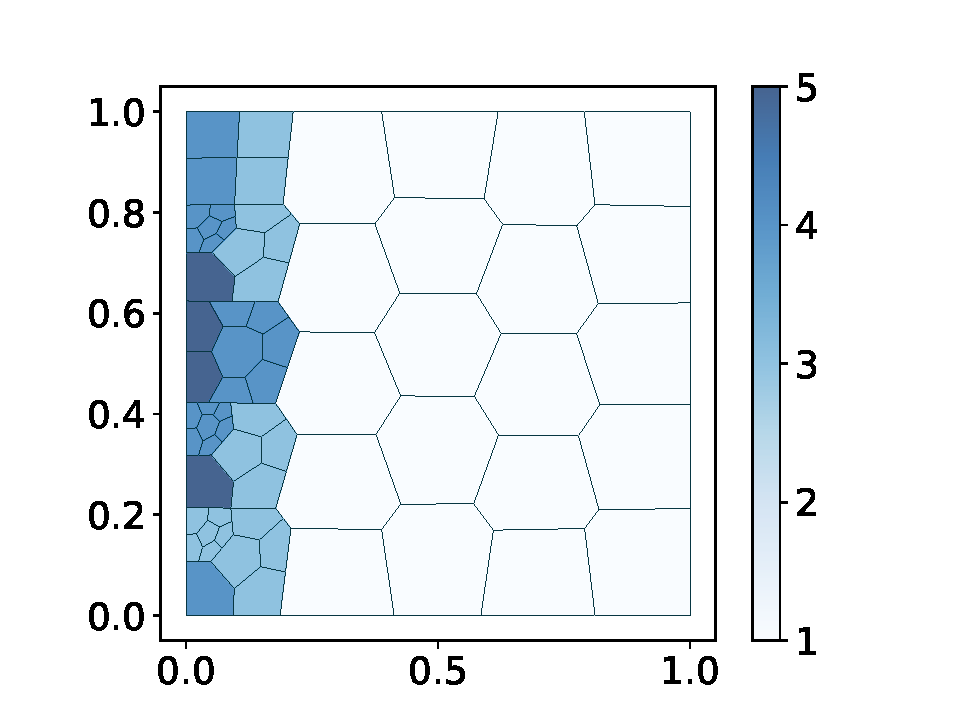
\includegraphics[trim=1cm 0.5cm 1cm 0.5cm, clip, width=0.275\textwidth]{meshes/adaptive/square_hp_1_5.pdf}
        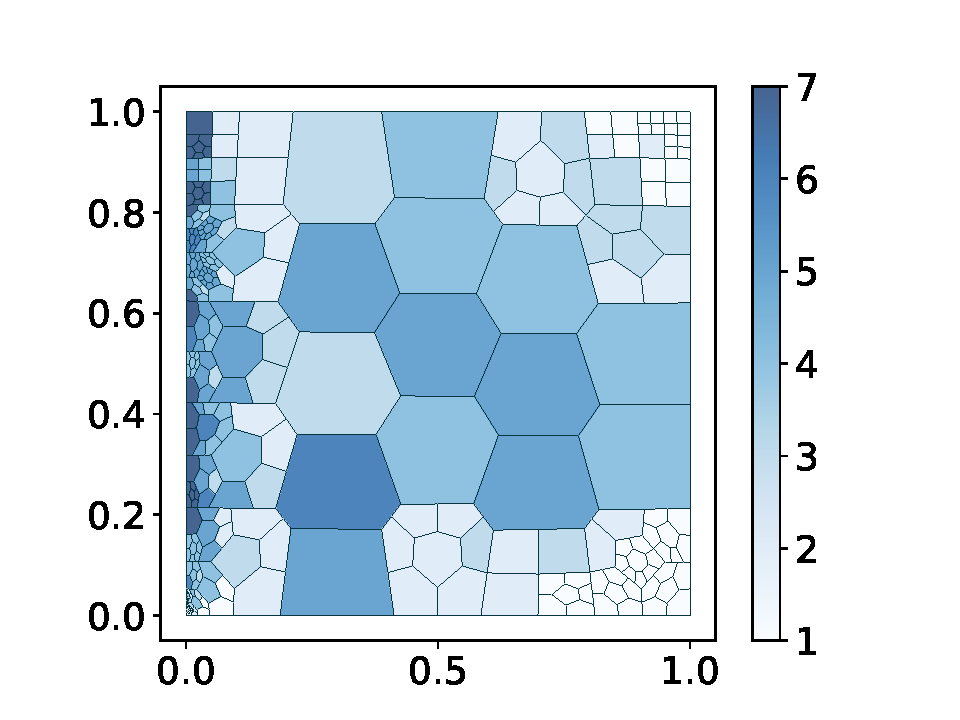
\includegraphics[trim=1cm 0.5cm 1cm 0.5cm, clip, width=0.275\textwidth]{meshes/adaptive/square_hp_1_10.pdf}
        \caption{Square mesh after 2, 5, and 10 refinements, $k_0 = 1$ and $N_0 = 25$.}
    \end{figure}
    
    \begin{figure}[!ht]
        \centering
        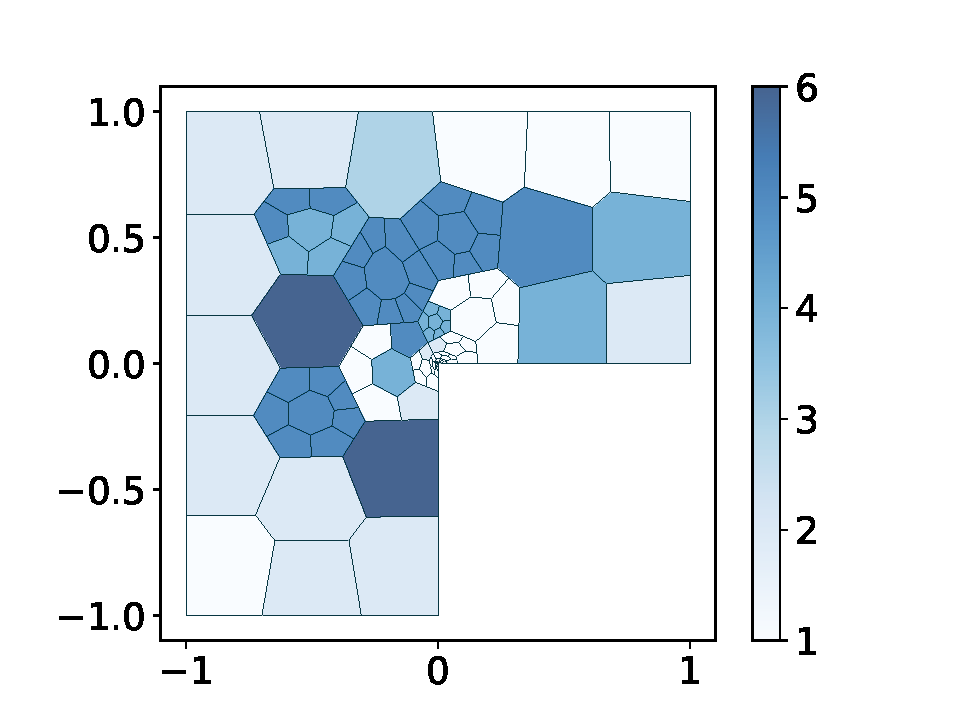
\includegraphics[trim=1cm 0.5cm 1cm 0.5cm, clip, width=0.275\textwidth]{meshes/adaptive/lshape_hp_1_5.pdf}
        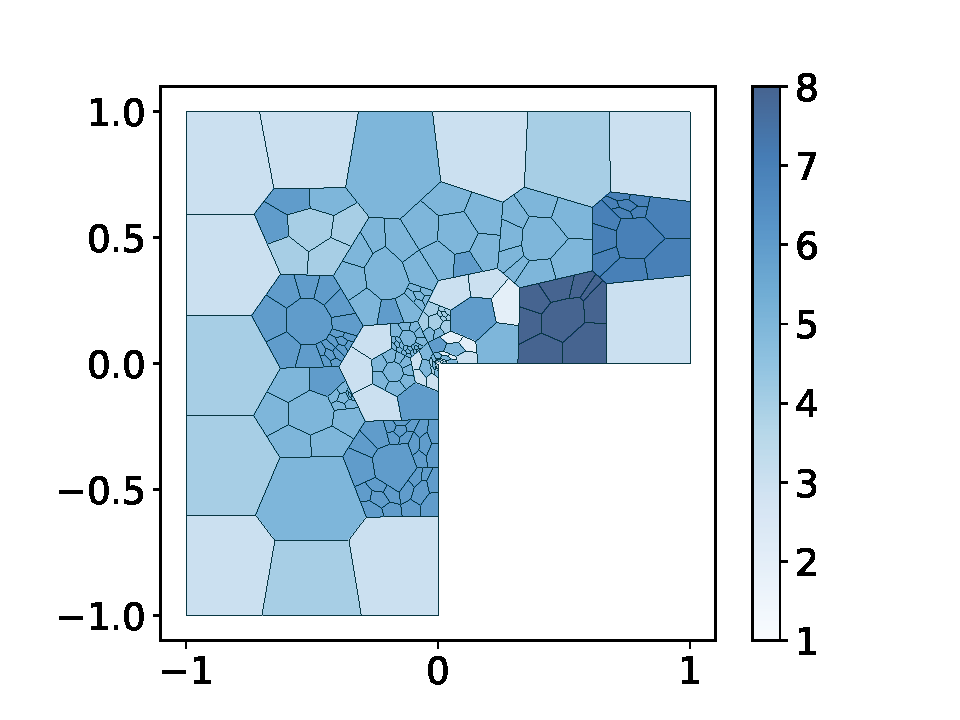
\includegraphics[trim=1cm 0.5cm 1cm 0.5cm, clip, width=0.275\textwidth]{meshes/adaptive/lshape_hp_1_10.pdf}
        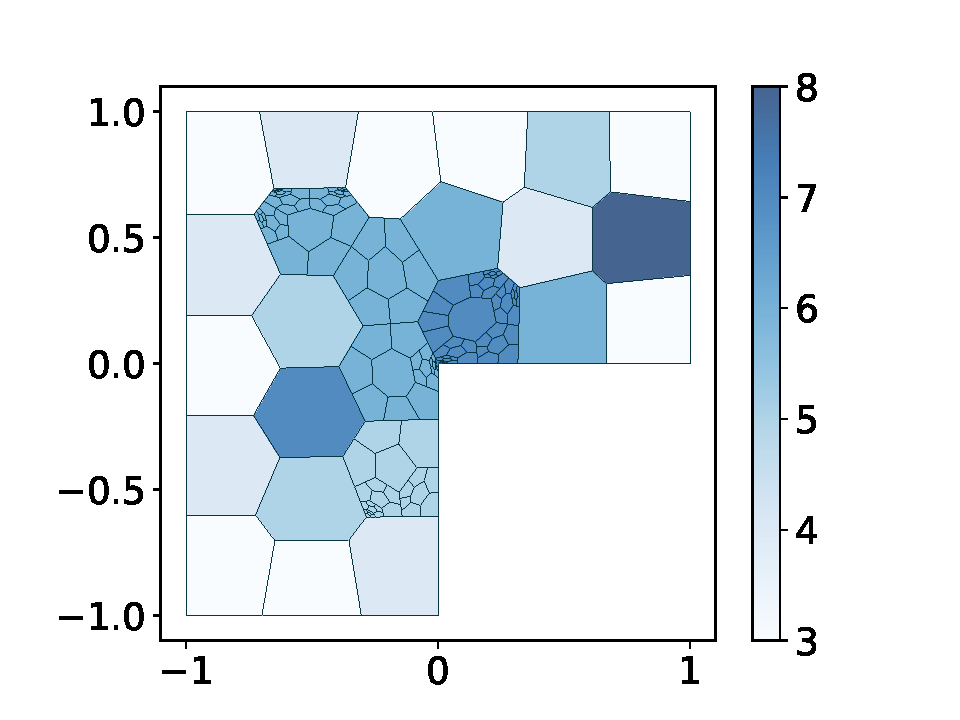
\includegraphics[trim=1cm 0.5cm 1cm 0.5cm, clip, width=0.275\textwidth]{meshes/adaptive/lshape_hp_1_15.pdf}
        \caption{L-shaped mesh after 5, 10, and 15 refinements, $k_0 = 1$ and $N_0 = 25$}
    \end{figure}
\end{frame}

\subsection{\textit{h-Adaptive} Refinement Versus \textit{hp-Adaptive} Refinement}

\begin{frame}[fragile]
    \frametitle{Errors}
    \framesubtitle{Both domains}

    \begin{figure}[!ht]
        \begin{subfigure}[b]{0.45\textwidth}
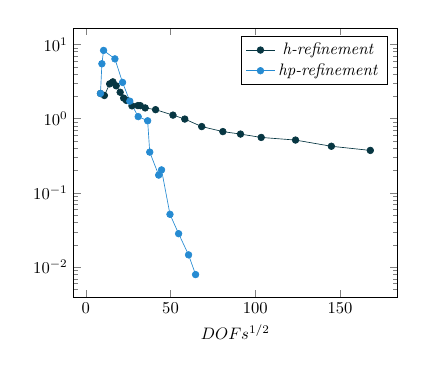
\begin{tikzpicture}[scale=.6]
\begin{axis}[
    xlabel={$DOFs^{1/2}$}, % Edit if needed.
    legend pos=north east,
    ymode=log
]

\addplot[solarized-base02, mark=*] coordinates {(8.660254037844387,2.1812) (10.954451150103322,2.04967) (14.071247279470288,2.93871) (15.968719422671311,3.13011) (17.916472867168917,2.76594) (20.273134932713294,2.26584) (22.315913604421397,1.89116) (23.93741840717165,1.76002) (27.2213151776324,1.48665) (30.740852297878796,1.49861) (32.17141588429082,1.49545) (35.02855977627399,1.39444) (41.1703777004778,1.3207) (51.43928459844674,1.11561) (58.40376700179535,0.986776) (68.38859554048467,0.782051) (80.87026647662292,0.669326) (91.27431182978046,0.619557) (103.50362312499017,0.558376) (123.75378782081783,0.514557) (144.9137674618944,0.424657) (167.88388844674762,0.373345)};
\addlegendentry{\textit{h-refinement}}

\addplot[\accentcolor, mark=*] coordinates {(8.660254037844387,2.1812) (9.486832980505138,5.48286) (10.488088481701515,8.28706) (17.175564037317667,6.37634) (21.6794833886788,3.07509) (25.96150997149434,1.71936) (30.903074280724887,1.06513) (36.4828726939094,0.935197) (37.72267222772003,0.3543) (43.0,0.173769) (44.68780594300866,0.204124) (49.66890375275057,0.0514923) (54.76312628037227,0.0282501) (60.63827174318213,0.0146515) (64.77653896280658,0.0079507)};
\addlegendentry{\textit{hp-refinement}}

\end{axis}
\end{tikzpicture}
\end{subfigure}
\hfill
\begin{subfigure}[b]{0.45\textwidth}
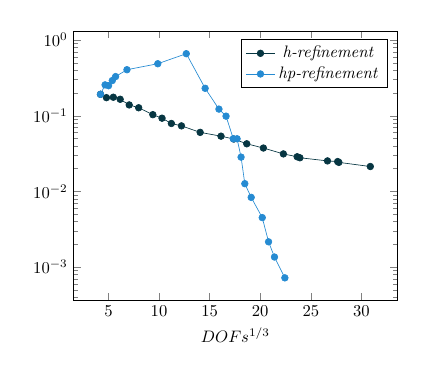
\begin{tikzpicture}[scale=.6]
\begin{axis}[
    xlabel={$DOFs^{1/3}$}, % Edit if needed.
    legend pos=north east,
    ymode=log
]

\addplot[solarized-base02, mark=*] coordinates {(4.217163326508746,0.191755) (4.805895533705332,0.173165) (5.484806552432618,0.17539) (6.162240147749038,0.164783) (7.054004063162272,0.138814) (7.989569740454012,0.127309) (9.39024187300355,0.103252) (10.297715269155368,0.0927241) (11.221408880627516,0.0789875) (12.21822948857921,0.073464) (14.067699311995325,0.0602545) (16.126599805218184,0.0536889) (17.386751706878687,0.0492177) (18.66925275961817,0.0425939) (20.31339680458661,0.0374376) (22.29090233304798,0.0313125) (23.651205489315725,0.028713) (23.918123773897065,0.0278557) (26.648390254618004,0.0253127) (27.653467034596552,0.0247917) (27.769363970258176,0.0242055) (30.87951848068366,0.0213387)};
\addlegendentry{\textit{h-refinement}}

\addplot[\accentcolor, mark=*] coordinates {(4.217163326508746,0.191755) (4.672328728355259,0.255398) (5.0132979349645845,0.248801) (5.383212612087283,0.291174) (5.708267473384861,0.328607) (6.832771452246442,0.404871) (9.878530490026034,0.485699) (12.69507321245234,0.659013) (14.55901434377428,0.230073) (15.921490395218942,0.122269) (16.623800957486996,0.098664) (17.340316055801914,0.0495985) (17.714635665253457,0.0495794) (18.10839938601742,0.0283923) (18.477938151928672,0.0126687) (19.10925056502305,0.00835058) (20.20211721754757,0.00451385) (20.823924640400417,0.00216312) (21.4106622851008,0.00136207) (22.436197851201577,0.00072339)};
\addlegendentry{\textit{hp-refinement}}

\end{axis}
\end{tikzpicture}
\end{subfigure}
        \caption{$DG$ error versus $DOFs^{1/2}$ (left) and $DOFs^{1/3}$ (right) on sequences of \textit{h-adaptively} (black) and \textit{hp-adaptively} (blue) refined meshes over a square (left) and an L-shaped domain (right). $k_0 = 1$, $N_0 = 25$.}
    \end{figure}
\end{frame}

	% References.
	\section*{References}
	\begin{frame}[allowframebreaks]
		\nocite{*}
		\printbibliography
	\end{frame}

	% Compiled on.
	\begin{frame}
		\thispagestyle{empty}
		\begin{center}
			Compiled on \today.
		\end{center}
	\end{frame}

\end{document}